\documentclass[12pt,t]{beamer}\usepackage[]{graphicx}\usepackage[]{color}
%% maxwidth is the original width if it is less than linewidth
%% otherwise use linewidth (to make sure the graphics do not exceed the margin)
\makeatletter
\def\maxwidth{ %
  \ifdim\Gin@nat@width>\linewidth
    \linewidth
  \else
    \Gin@nat@width
  \fi
}
\makeatother

\definecolor{fgcolor}{rgb}{0.345, 0.345, 0.345}
\newcommand{\hlnum}[1]{\textcolor[rgb]{0.686,0.059,0.569}{#1}}%
\newcommand{\hlstr}[1]{\textcolor[rgb]{0.192,0.494,0.8}{#1}}%
\newcommand{\hlcom}[1]{\textcolor[rgb]{0.678,0.584,0.686}{\textit{#1}}}%
\newcommand{\hlopt}[1]{\textcolor[rgb]{0,0,0}{#1}}%
\newcommand{\hlstd}[1]{\textcolor[rgb]{0.345,0.345,0.345}{#1}}%
\newcommand{\hlkwa}[1]{\textcolor[rgb]{0.161,0.373,0.58}{\textbf{#1}}}%
\newcommand{\hlkwb}[1]{\textcolor[rgb]{0.69,0.353,0.396}{#1}}%
\newcommand{\hlkwc}[1]{\textcolor[rgb]{0.333,0.667,0.333}{#1}}%
\newcommand{\hlkwd}[1]{\textcolor[rgb]{0.737,0.353,0.396}{\textbf{#1}}}%
\let\hlipl\hlkwb

\usepackage{framed}
\makeatletter
\newenvironment{kframe}{%
 \def\at@end@of@kframe{}%
 \ifinner\ifhmode%
  \def\at@end@of@kframe{\end{minipage}}%
  \begin{minipage}{\columnwidth}%
 \fi\fi%
 \def\FrameCommand##1{\hskip\@totalleftmargin \hskip-\fboxsep
 \colorbox{shadecolor}{##1}\hskip-\fboxsep
     % There is no \\@totalrightmargin, so:
     \hskip-\linewidth \hskip-\@totalleftmargin \hskip\columnwidth}%
 \MakeFramed {\advance\hsize-\width
   \@totalleftmargin\z@ \linewidth\hsize
   \@setminipage}}%
 {\par\unskip\endMakeFramed%
 \at@end@of@kframe}
\makeatother

\definecolor{shadecolor}{rgb}{.97, .97, .97}
\definecolor{messagecolor}{rgb}{0, 0, 0}
\definecolor{warningcolor}{rgb}{1, 0, 1}
\definecolor{errorcolor}{rgb}{1, 0, 0}
\newenvironment{knitrout}{}{} % an empty environment to be redefined in TeX

\usepackage{alltt}
% \documentclass[t]{beamer}

\usepackage{pgfpages}
\usepackage{pgffor}
%\pgfpagesuselayout{4 on 1}[a4paper,landscape]

%\pagestyle{empty} % descomentar para impresión muy blanca

\usepackage[utf8]{inputenc}
\usepackage[spanish]{babel}
\usepackage{verbatim}
\usepackage{hyperref}
\usepackage{amsfonts,amssymb,amsmath,amsthm, wasysym}
\usepackage{listings}
\usepackage[T1]{fontenc}        
\usepackage{pgf}
%\usepackage{epsdice}
\usepackage{pgfpages}
\usepackage{tikz}
%\usetikzlibrary{arrows,shapes,plotmarks,backgrounds,trees,positioning}
%\usetikzlibrary{decorations.pathmorphing,calc,snakes}
%\usepackage{marvosym}
%
\usetheme[hideothersubsections,left]{Marburg}
\usecolortheme{sidebartab}
\useinnertheme[shadow]{rounded}
% \useoutertheme[footline=empty,subsection=true,compress]{infolines}
% \useoutertheme[footline=empty,subsection=true,compress]{miniframes}
% \usefonttheme{serif}

\setbeamertemplate{caption}[numbered]
\setbeamertemplate{navigation symbols}{}


\newcommand{\red}[1]{\textcolor{red}{#1}}
\newcommand{\green}[1]{\textcolor{green}{#1}}
\newcommand{\blue}[1]{\textcolor{blue}{#1}}
\newcommand{\gray}[1]{\textcolor{gray}{#1}}
\renewcommand{\emph}[1]{{\color{red}#1}}

\setbeamertemplate{frametitle}
{\begin{centering}
\medskip
\color{blue}
\textbf{\insertframetitle}
\medskip
\end{centering}
}
\usecolortheme{rose}
\usecolortheme{dolphin}
\mode<presentation>


\newcommand{\CC}{\mathbb{C}}
\newcommand{\RR}{\mathbb{R}}
\newcommand{\ZZ}{\mathbb{Z}}
\newcommand{\NN}{\mathbb{N}}
\newcommand{\KK}{\mathbb{K}}
\newcommand{\MM}{\mathcal{M}}
%\newcommand{\dbinom}{\displaystyle\binom}

\newcommand{\limn}{{\displaystyle \lim_{n\to\infty}}}
\renewcommand{\leq}{\leqslant}
\renewcommand{\geq}{\geqslant}
\def\tendeix{{\displaystyle\mathop{\longrightarrow}_{\scriptscriptstyle
n\to\infty}}}

\newcommand{\matriu}[1]{\left(\begin{matrix} #1 \end{matrix}\right)}

% \newcommand{\qed}{\hbox{}\nobreak\hfill\vrule width 1.4mm height 1.4mm depth 0mm
%     \par \goodbreak \smallskip}
%
% %
\theoremstyle{plain}
\newtheorem{teorema}{Teorema}
\newtheorem{prop}{Proposición}
\newtheorem{cor}{Corolario}
\theoremstyle{definition}
\newtheorem{Ejemplo}{Ejemplo}
\newtheorem{exerc}{Ejercicio}
\newtheorem{defin}{Definición}
\newtheorem{obs}{Observación}

\newcounter{seccions}
\newcommand{\seccio}[1]{\addtocounter{seccions}{1}
\medskip\par\noindent\textbf{\theseccions.
#1}\smallskip\par }

\newcommand{\EM}{\Omega}
\newcommand{\PP}{\mathcal{P}}

\title[\red{Matemáticas III GINF}]{}
\author[]{}
\date{}
\IfFileExists{upquote.sty}{\usepackage{upquote}}{}
\begin{document}
\beamertemplatedotitem

\lstset{backgroundcolor=\color{green!50}}
\lstset{breaklines=true}
\lstset{basicstyle=\ttfamily}


\section{Estimación puntual}

\begin{frame}
\vfill
\begin{center}
\gray{\LARGE Estimación por intervalos}
\end{center}
\vfill
\end{frame}


\section{Estimación por Intervalos}

\begin{frame}
\vfill
\begin{center}
\gray{\LARGE Estimación por Intervalos}
\end{center}
\vfill
\end{frame}

\subsection{Definiciones básicas}

\begin{frame}
\frametitle{El problema}
\vspace*{-1cm}

\begin{center}
\hspace*{-0.6cm}

\includegraphics[width=1.1\linewidth]{sanidade}
\end{center}
\vspace*{-1ex}

Con un estimador, estimamos el parámetro con una cierta precisión, que depende:
\medskip

\begin{itemize}
\item De la variabilidad del estimador
\medskip

\item Del tamaño de la muestra
\medskip

\item Del \emph{nivel de confianza} de la  estimación: cuan seguros  queremos estar de que la estimación es correcta
\end{itemize}
\end{frame}



\begin{frame}
\frametitle{El problema}
\vspace*{-1cm}

\begin{center}
\hspace*{-0.5cm}

\includegraphics[width=1.1\linewidth]{plagiUIB1.jpg}\medskip

\hspace*{-0.4cm}

\includegraphics[width=1.05\linewidth]{plagiUIB3.jpg}\medskip

\hspace*{-0.5cm}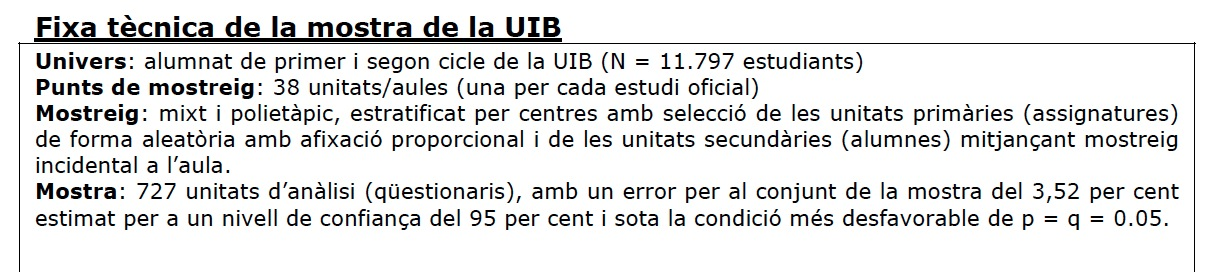
\includegraphics[width=1.1\linewidth]{plagiUIB2.jpg}
\end{center}
\vspace*{-1ex}

Por lo tanto ( y por el momento):
\begin{quote}
\red{Con 95\% de confianza podemos afirmar que entre un 73.1\% y un 80.1\% de los estudiantes de la UIB aceptan \ldots}
\end{quote}
\end{frame}


\begin{frame}
\frametitle{El problema}
\vspace*{-0.5cm}

\begin{center}

\includegraphics[width=1\linewidth]{EPA3}
\end{center}
\end{frame}

\begin{frame}
\frametitle{Definiciones básicas}

En la \blue{Encuesta de Población Activa} (\blue{EPA}):

\begin{center}
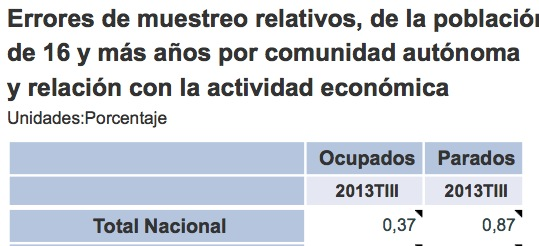
\includegraphics[width=0.6\linewidth]{EPA1}

{\scriptsize \url{http://www.ine.es/jaxi/tabla.do?per=03&type=db&divi=EPA&idtab=313}}
\medskip

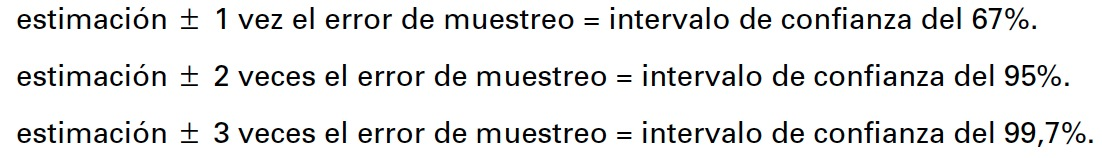
\includegraphics[width=\linewidth]{EPA2}


{\scriptsize \url{http://www.ine.es/docutrab/eval_epa/evaluacion_epa04.pdf}}
\end{center}
\end{frame}

\begin{frame}
\frametitle{El problema}
\vspace*{-2ex}

\blue{EPA de octubre de 2013}: \smallskip
\begin{itemize}
\item El número  estimado de parados a nivel nacional fue del  5\,904\,700 \smallskip

\item El error de muestreo fue de un 0.87\% \smallskip

\item Por lo tanto, estamos bastante seguros (nivel de confianza del 95\%) de que el número de parados estaba entre
$$
\begin{array}{rl}
\hspace*{-2ex} 5\,904\,700\!-\! 2\!\cdot \! 0.0087\!\cdot\! 5\,904\,700 & \hspace*{-1ex}=\! 5\,904\,700\!-\! 102\,742\\ &  \hspace*{-1ex}=\! 5\,801\,958\quad \mbox{ y}\\
\hspace*{-2ex} 5\,904\,700\!+\!2\!\cdot\! 0.0087\!\cdot\! 5\,904\,700 & \hspace*{-1ex}=\! 5\,904\,700\!+\! 102\,742\\ & \hspace*{-1ex}=\! 6\,007\,442
 \end{array}
 $$
 
 \item La EPA de junio del 2013 había estimado el número de parados  en  5\,977\,500
 \smallskip
 
 \item \red{No hay evidencia de que  el paro bajase}
 \end{itemize}
\end{frame}


\begin{frame}
\frametitle{Definiciones básicas}

Una \emph{estimación por intervalos} de un parámetro poblacional es una regla para calcular, a partir de una muestra, un intervalo en el que, con una cierta probabilidad (\emph{nivel de confianza}), se encuentra el  valor verdadero del parámetro
\bigskip

Estas reglas definirán,  a su vez, \emph{estimadores}

\end{frame}



\begin{frame}
\frametitle{Ejemplos}


\blue{Ejemplo:} 
Hemos escogido al azar 50 estudiantes de grado de la UIB, hemos calculada sus notas medias de las asignaturas del primer semestre, y la media de estas medias ha sido un 6.3, con una varianza muestral de 1.8.\medskip

Determinar un intervalo del que podamos afirmar con probabilidad 95\% que contiene la media real de las notas medias de los estudiantes de grado de la UIB este primer semestre.
\end{frame}


\begin{frame}
\frametitle{Ejemplos}


\blue{Ejemplo:} En un experimento se ha medido el porcentaje de aumento de alcohol en sangre a 40 personas despuesde tomar 4 cañas de cerveza. La media y la desviación típica muestral de estos porcentajes de incremento han sido
$$
\overline{x}=41.2,\quad \widetilde{s}=2.1
$$
Determinar un intervalo que podamos afirmar con probabilidad 95 \% que contiene el porcentaje de aumento medio de alcohol en sangre (verdadero) de una persona despuesde beber cuatro cañas de cerveza.
\end{frame}




\begin{frame}
\frametitle{Definiciones básicas}

Dado un parámetro $\theta$, el intervalo $]A,B[$ es un \emph{intervalo de confianza} del
$(1-\alpha)\cdot 100\% $ para al parámetro $\theta$ cuando
$$
P(A<\theta<B)=1-\alpha
$$
El valor $(1-\alpha)\cdot 100\% $ (o contiene solo el $1-\alpha$) recibe el nombre de \emph{nivel de confianza} 
\medskip

El valor $\alpha$ recibe el nombre de \emph{nivel de significación}
\medskip 


\blue{Ejemplo:} $]A,B[$ es un intervalo de confianza del $95\%$ (o de nivel de significación de 0.05) si
$$
P(A<\theta<B)=0.95
$$


\end{frame}




\begin{frame}
\frametitle{Definiciones básicas}

\emph{Por defecto}, buscaremos  intervalos tales que la \emph{cola} de probabilidad sobrante $\alpha$ se reparta por igual a cada lado  del intervalo:
$$
P(\theta<A)=P(\theta>B)=\frac{\alpha}{2}
$$
\begin{center}
\begin{tikzpicture}[thick,scale=0.8]%[>=stealth]%,yscale=0.5,xscale=0.7]
\draw (0,0)--(10,0);
\draw (3,0.3)--(3,-0.3);
\draw (7,0.3)--(7,-0.3);
\draw(3,-0.6) node {\small $A$}; 
\draw (7,-0.6) node {\small $B$}; 
\draw[red] (8.5,-0.3) node {\small $\alpha/2$}; 
\draw[red] (1.5,-0.3) node {\small $\alpha/2$}; 
\draw[red] (5,-0.3) node {\small $1-\alpha$}; 
\end{tikzpicture}
\end{center}


\blue{Ejemplo:} Para buscar  un intervalo de confianza  $]A,B[$ del $95\%$, buscaremos $A,B$ de manera que 
$$
P(\theta<A)=0.025\quad\mbox{ y }\quad P(\theta>B)=0.025
$$


\end{frame}

\subsection{$\mu$ de población normal con $\sigma$ conocida}
\begin{frame}
\frametitle{Ejemplo: $\mu$ de población normal con $\sigma$ conocida}

Sea $X$ una v.a. normal con media poblacional $\mu$ desconocida y desviación típica poblacional $\sigma$ conocida (a la práctica, usualmente, \emph{estimada en un experimento anterior})
\medskip

Sea $X_1,\ldots,X_n$ una m.a.s. de $X$, con media muestral $\overline{X}$
\medskip

Queremos determinar un intervalo de confianza para a $\mu$ con un cierto nivel de confianza (digamos, 97.5\%):  un intervalo $]A,B[$ tal que
$$
P(A<\mu<B)=0.975
$$


\end{frame}

\begin{frame}
\frametitle{Ejemplo: $\mu$ de población normal con $\sigma$ conocida}

Bajo estas  condiciones, sabemos que 
$$
Z=\frac{\overline{X}-\mu}{\sigma/\sqrt{n}}
$$
sigue una distribuciónn normal estándar
\medskip

Comencemos calculando un intervalo centrado en $0$ en el que   $Z$ 
tenga probabilidad $0.975$:
$$
\begin{array}{l}
0.975\!=\! P(-\delta<Z<\delta)\!=\!F_{Z}(\delta)\!-\!F_{Z}(-\delta)\!=\!
2 F_{Z}(\delta)\!-\!1\\[2ex]
F_{Z}(\delta)=\dfrac{1.975}{2}=0.9875\Rightarrow
\delta=\texttt{qnorm(0.9875)}=2.24
\end{array}
$$
\end{frame}


\begin{frame}
\frametitle{Ejemplo: $\mu$ de población normal con $\sigma$ conocida}
Por lo tanto
$$
P(-2.24<Z<2.24)=0.975
$$
Substituyendo $Z=\dfrac{\overline{X}-\mu}{\sigma/\sqrt{n}}$
$$
\begin{array}{c}
P\left(-2.24<\dfrac{\overline{X}-\mu}{\sigma/\sqrt{n}}
<2.24\right)=0.975\\[3ex]
P\left(\overline{X} -2.24 \dfrac{\sigma}{\sqrt{n}}< \mu< \overline{X}+
2.24\dfrac{\sigma}{\sqrt{n}}\right)=0.975
\end{array}
$$
\end{frame}

\begin{frame}
\frametitle{Ejemplo: $\mu$ de població normal con $\sigma$ conocida}
Por  lo tant, la probabilidad que la media  $\mu$ de $X$ 
se encuentre dentro del intevalo
$$
\left]\overline{X} -2.24 \frac{\sigma}{\sqrt{n}},
\overline{X}+ 2.24\frac{\sigma}{\sqrt{n}}
\right[
$$
es $0.975$: es un intervalo de confianza  del 97.5\%
\pause\medskip

\red{Además tenemos que:}
\begin{itemize}
\item Está centrado en $\overline{X}$
\medskip

\item El 0.025 de probabilidad restante  está repartido por igual en los dos extremos del intervalo
\end{itemize}
\end{frame}

\begin{frame}
\frametitle{Ejemplo: $\mu$ de població normal con $\sigma$ conocida}


\begin{itemize}
\item \blue{Como  estimador:} Un 97.5\% de las veces  que tomemos una muestra de tamaño $n$ de $X$, el verdadero valor de $\mu$ caerá dentro de este intervalo 
\medskip

\item \blue{Para una mostra concreta:} La probabilidad que, si  una $\mu$ ha producido esta mostra, esté en este intervalo concreto, es del 97.5\%
\medskip

\item \blue{En ocasiones lo entenderemos como}:  ``La probabilidad de que $\mu$ esté en este intervalo  es del 97.5\%''
\medskip

\item \blue{Pero no la frease anterio es mentira} (\emph{es un abusio de lenguaje}): La $\mu$ concreta es un valor fijo, por lo  tanto  que pertenezca o   no a aquest intervalo concreto tiene probabilidad 1 (si hi pertenece) y 0 (si no  pertenece) 
\end{itemize}


\end{frame}



\begin{frame}
\frametitle{I.C. pera $\mu$ de población normal con $\sigma$ conocida}
\vspace*{-3ex}

\begin{teorema}
Sea $X\sim N(\mu,\sigma)$ con $\mu$ desconocida y $\sigma$ conocida.
\medskip

Tomamos una m.a.s. de $X$ de medida $n$, con media $\overline{X}$.
\medskip

Un intervalo de confianza  del $(1-\alpha)\cdot 100\%$ pera $\mu$  es
$$
\left]\overline{X} -z_{1-\frac{\alpha}{2}} \frac{\sigma}{\sqrt{n}}, \overline{X}+z_{1-\frac{\alpha}{2}}\frac{\sigma}{\sqrt{n}}
\right[
$$
donde $z_{1-\frac{\alpha}{2}}$ es el $(1-\frac{\alpha}{2})$-cuantil de la normal  estándard $Z$ (es decir, $z_{1-\frac{\alpha}{2}}=F_Z^{-1}(1-\frac{\alpha}{2})$, o $P(Z\leq z_{1-\frac{\alpha}{2}})=1-\frac{\alpha}{2}$)
\end{teorema}

%(Recordau que $F_Z^{-1}(\frac{\alpha}{2})=-F_Z^{-1}(1-\frac{\alpha}{2})$)

\end{frame}


\begin{frame}
\frametitle{I.C. para $\mu$ de población normal con $\sigma$ conocida}

Si $X$ es normal con $\sigma$ conocida, un intervalo de confianza  I.C. para $\mu$ de población normal con $\sigma$ conocida $\mu$ del $(1-\alpha)\cdot 100\%$ es
$$
\red{\overline{X} \pm z_{1-\frac{\alpha}{2}} \frac{\sigma}{\sqrt{n}}}:=\left]\overline{X} -z_{1-\frac{\alpha}{2}} \frac{\sigma}{\sqrt{n}}, \overline{X}+z_{1-\frac{\alpha}{2}}\frac{\sigma}{\sqrt{n}}
\right[
$$
Observad que está centrado   en $\overline{X}$
\begin{center}
\begin{tabular}{c|c|c}
\blue{confianza  $1-\alpha$} & \blue{Significación $\alpha$} & \blue{$z_{1-\frac{\alpha}{2}}$}\\
 \hline
0.900\ & 0.100 &1.64 \\   
0.950 & 0.050 & 1.96\\
0.975 & 0.025 & 2.24 \\
0.990 & 0.010 & 2.58
\end{tabular}
\end{center}

\end{frame}

\begin{frame}[fragile]
\frametitle{I.C. para $\mu$ de población normal con $\sigma$ conocida}
\vspace*{-4ex}

\begin{knitrout}\footnotesize
\definecolor{shadecolor}{rgb}{0.969, 0.969, 0.969}\color{fgcolor}\begin{kframe}
\begin{alltt}
\hlstd{ICZ}\hlkwb{=}\hlkwa{function}\hlstd{(}\hlkwc{x}\hlstd{,}\hlkwc{sigma}\hlstd{,}\hlkwc{alpha}\hlstd{)\{}
  \hlkwd{c}\hlstd{(}\hlkwd{mean}\hlstd{(x)}\hlopt{-}\hlkwd{qnorm}\hlstd{(}\hlnum{1}\hlopt{-}\hlstd{alpha}\hlopt{/}\hlnum{2}\hlstd{)}\hlopt{*}\hlstd{sigma}\hlopt{/}\hlkwd{sqrt}\hlstd{(}\hlkwd{length}\hlstd{(x)),}
  \hlkwd{mean}\hlstd{(x)}\hlopt{+}\hlkwd{qnorm}\hlstd{(}\hlnum{1}\hlopt{-}\hlstd{alpha}\hlopt{/}\hlnum{2}\hlstd{)}\hlopt{*}\hlstd{sigma}\hlopt{/}\hlkwd{sqrt}\hlstd{(}\hlkwd{length}\hlstd{(x)))\}}
\hlkwd{set.seed}\hlstd{(}\hlnum{5}\hlstd{)}
\hlstd{mu}\hlkwb{=}\hlnum{1.5}\hlstd{; sigma}\hlkwb{=}\hlnum{1}\hlstd{; alpha}\hlkwb{=}\hlnum{0.05}
\hlstd{Poblacion}\hlkwb{=}\hlkwd{rnorm}\hlstd{(}\hlnum{10}\hlopt{^}\hlnum{6}\hlstd{,mu,sigma)}
\hlstd{M}\hlkwb{=}\hlkwd{replicate}\hlstd{(}\hlnum{100}\hlstd{,}\hlkwd{ICZ}\hlstd{(}\hlkwd{sample}\hlstd{(Poblacion,}\hlnum{50}\hlstd{,}\hlkwc{replace}\hlstd{=T),}
 \hlstd{sigma,alpha))}
\hlkwd{plot}\hlstd{(}\hlnum{1}\hlopt{:}\hlnum{10}\hlstd{,}\hlkwc{type}\hlstd{=}\hlstr{"n"}\hlstd{,}\hlkwc{xlim}\hlstd{=}\hlkwd{c}\hlstd{(}\hlnum{1.2}\hlstd{,}\hlnum{1.8}\hlstd{),}\hlkwc{ylim}\hlstd{=}\hlkwd{c}\hlstd{(}\hlnum{0}\hlstd{,}\hlnum{100}\hlstd{),}
\hlkwc{xlab}\hlstd{=}\hlstr{"Valores"}\hlstd{,}\hlkwc{ylab}\hlstd{=}\hlstr{"Replicaciones"}\hlstd{)}
\hlstd{seg.int}\hlkwb{=}\hlkwa{function}\hlstd{(}\hlkwc{i}\hlstd{)\{color}\hlkwb{=}\hlstr{"grey"}\hlstd{;}
  \hlkwa{if}\hlstd{((mu}\hlopt{<}\hlstd{M[}\hlnum{1}\hlstd{,i])} \hlopt{|} \hlstd{(mu}\hlopt{>}\hlstd{M[}\hlnum{2}\hlstd{,i]))\{color} \hlkwb{=} \hlstr{"red"}\hlstd{\}}
  \hlkwd{segments}\hlstd{(M[}\hlnum{1}\hlstd{,i],i,M[}\hlnum{2}\hlstd{,i],i,}\hlkwc{col}\hlstd{=color,}\hlkwc{lwd}\hlstd{=}\hlnum{3}\hlstd{)\}}
\hlkwd{invisible}\hlstd{(}\hlkwd{sapply}\hlstd{(}\hlnum{1}\hlopt{:}\hlnum{100}\hlstd{,}\hlkwc{FUN}\hlstd{=seg.int))}
\hlkwd{abline}\hlstd{(}\hlkwc{v}\hlstd{=mu,}\hlkwc{lwd}\hlstd{=}\hlnum{3}\hlstd{)}
\end{alltt}
\end{kframe}
\end{knitrout}

\end{frame}

\begin{frame}

\frametitle{I.C. para $\mu$ de población normal con $\sigma$ conocida}
\vspace*{-1cm}

% \begin{center}
% 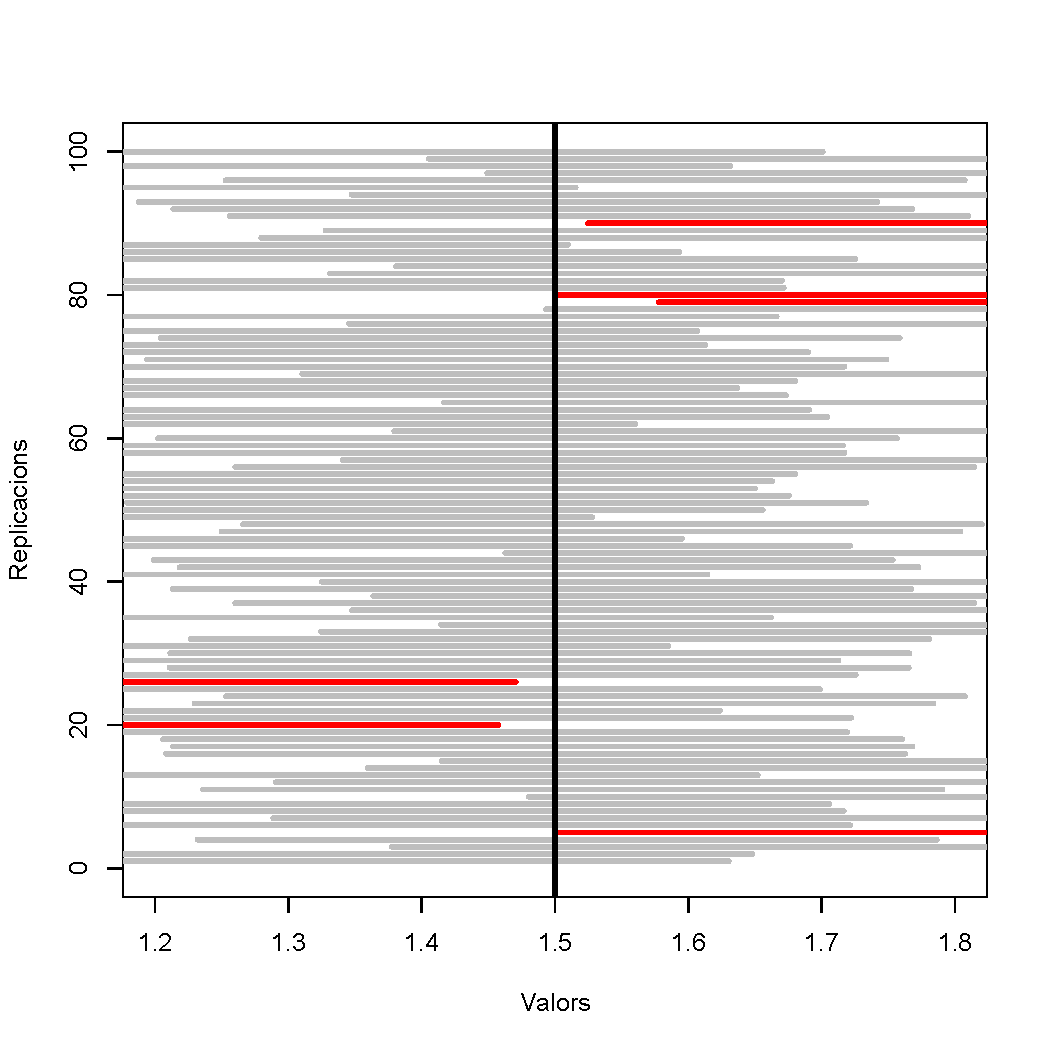
\includegraphics[width=0.9\linewidth]{intervals1}
% \end{center}
\begin{knitrout}
\definecolor{shadecolor}{rgb}{0.969, 0.969, 0.969}\color{fgcolor}
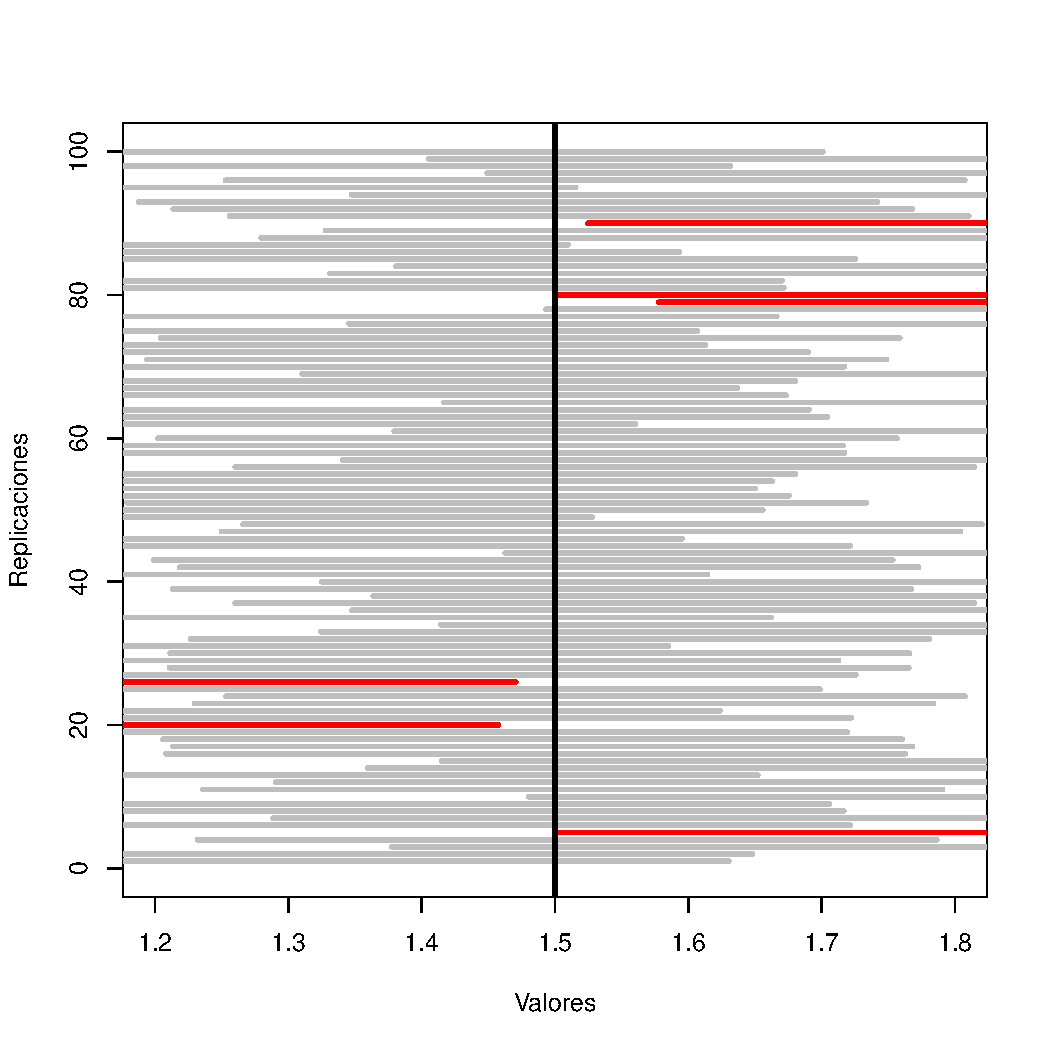
\includegraphics[width=0.9\linewidth]{figure/plot_intervalos-1} 

\end{knitrout}




\end{frame}

\begin{frame}[fragile]
\frametitle{I.C. para $\mu$ de población normal con $\sigma$ conocida}

\begin{block}{\red{¡Atención!}}
De media, un $\alpha100\%$ de las veces, un intervalo de confianza  del $(1-\alpha)100\%$  no contendrá el valor real del parámetro 
\end{block}

\blue{Ejemplo}: De media, un 5\% de las vegades un intervalo de confianza  del 95\% no contendrá el valor real del parámetro

\end{frame}




\begin{frame}
\frametitle{Ejemplo}
\red{$\displaystyle
\left]\overline{X} -z_{1-\frac{\alpha}{2}} \frac{\sigma}{\sqrt{n}}, \overline{X}+z_{1-\frac{\alpha}{2}}\frac{\sigma}{\sqrt{n}}
\right[$}
\medskip


Tomamos una m.a.s. de  tamaño  $n=16$ de una v.a. normal con $\sigma=4$ y $\mu$ desconocida. La media   de la m.a.s. es
$\overline{x}=20$.
\medskip

\blue{Calculad un intervalo de confianza  del 97.5\%  para $\mu$ de  una población normal con $\sigma$ conocida$\mu$}
\pause
$$
\left] 20-2.24\cdot \frac{4}{\sqrt{16}} ,
20+2.24\cdot \frac{4}{\sqrt{16}}
\right[
=]17.76,22.24[
$$

La probabilidad que un parámetro $\mu$ que haya producido la muestra esté en este intervalo  es $0.975$
\pause\medskip

\textsl{``La probabilidad que el parámetro $\mu$  de la población que ha producido la muestra este  en este intervalo  es $0.975$''}


\end{frame}

%\end{document}

\begin{frame}[fragile]
\frametitle{Ejemplo}
Queremos que analizar un sensor que mide la temperatura de un procesador en grados centígrados \footnote{En concreto un \emph{Intel Core i7-2600K}} que tiene 	como temperatura normal de  $32^{\circ}$ a $40^{\circ}$. Para saber si está bien calibrado, diseñamos un experimento en el que ponemos  el procesador el procesador en las mismas condiciones y  tomamos 40 muestras de su temperatura.
Los resultados son los Seaentes:

\begin{knitrout}\small
\definecolor{shadecolor}{rgb}{0.969, 0.969, 0.969}\color{fgcolor}\begin{kframe}
\begin{alltt}
\hlstd{temperatura}\hlkwb{=}\hlkwd{c}\hlstd{(}\hlnum{36}\hlstd{,}\hlnum{35}\hlstd{,}\hlnum{38}\hlstd{,}\hlnum{38}\hlstd{,}\hlnum{36}\hlstd{,}\hlnum{37}\hlstd{,}\hlnum{38}\hlstd{,}\hlnum{36}\hlstd{,}\hlnum{37}\hlstd{,}\hlnum{36}\hlstd{,}
              \hlnum{37}\hlstd{,}\hlnum{37}\hlstd{,}\hlnum{34}\hlstd{,}\hlnum{38}\hlstd{,}\hlnum{35}\hlstd{,}\hlnum{37}\hlstd{,}\hlnum{36}\hlstd{,}\hlnum{36}\hlstd{,}\hlnum{34}\hlstd{,}\hlnum{38}\hlstd{,}
              \hlnum{36}\hlstd{,}\hlnum{37}\hlstd{,}\hlnum{35}\hlstd{,}\hlnum{35}\hlstd{,}\hlnum{35}\hlstd{,}\hlnum{35}\hlstd{,}\hlnum{36}\hlstd{,}\hlnum{36}\hlstd{,}\hlnum{36}\hlstd{,}\hlnum{35}\hlstd{,}
              \hlnum{36}\hlstd{,}\hlnum{35}\hlstd{,}\hlnum{34}\hlstd{,}\hlnum{34}\hlstd{,}\hlnum{37}\hlstd{,}\hlnum{37}\hlstd{,}\hlnum{35}\hlstd{,}\hlnum{36}\hlstd{,}\hlnum{34}\hlstd{,}\hlnum{36}\hlstd{)}
\hlkwd{mean}\hlstd{(temperatura)}
\end{alltt}
\begin{verbatim}
## [1] 35.975
\end{verbatim}
\end{kframe}
\end{knitrout}

\end{frame}
%\end{document}
\begin{frame}[fragile]
\frametitle{Ejemplo}
\vspace*{-3ex}

\blue{Supongamos  que las medidas de nuestro sensor siguen  una distribuciónn normal con varianza poblacional conocida $\sigma^2=1.44$. Calculad un intervalo de confianza  del 90\% para al resultado medio de la temperatura del procesador.}
%\pause
\medskip

Tenemos las Seaentes condiciones:
\begin{itemize}
\item Población normal con $\sigma=\sqrt{1.44}=1.2$ conocida
\item M.a.s. de  tamaño  $n=40$
\item media de la muestra  $\overline{x}=35.975$
\item $1-\alpha=0.9\Rightarrow \alpha=0.1\Rightarrow 1-\frac{\alpha}{2}=0.95$
\item $z_{0.95}\approx 1.64$
\begin{itemize}
\item Con la tabla de $Z$, $P(Z\leq 1.64)=0.9495\approx 0.95$
\item Con R
\begin{knitrout}
\definecolor{shadecolor}{rgb}{0.969, 0.969, 0.969}\color{fgcolor}\begin{kframe}
\begin{alltt}
\hlkwd{qnorm}\hlstd{(}\hlnum{0.95}\hlstd{)}
\end{alltt}
\begin{verbatim}
## [1] 1.644854
\end{verbatim}
\end{kframe}
\end{knitrout}
\end{itemize}
\end{itemize}

\end{frame}


\begin{frame}
\frametitle{Ejemplo}
Aplicamos la fórmula
$$
\overline{X}\pm z_{1-\frac{\alpha}{2}} \frac{\sigma}{\sqrt{n}}
$$
con
$$
\overline{x}=35.975, z_{0.95}=1.64, \sigma=\sqrt{1.44}=1.2, n=40
$$

Obtenemos que el intervalo de confianza  del 90\% pedido es 

$$
35.975\pm 1.64\cdot\frac{1.2}{\sqrt{40}}=
]34.991 , 36.959[
$$

\end{frame}


\begin{frame}
\frametitle{Amplitud}

La \emph{amplitud} $A$ de un intervalo de confianza  
$$
\left]\overline{X} -z_{1-\frac{\alpha}{2}} \frac{\sigma}{\sqrt{n}}, \overline{X}+z_{1-\frac{\alpha}{2}}\frac{\sigma}{\sqrt{n}}
\right[
$$
es
$$
\begin{array}{rl}
\red{A}& \displaystyle =\overline{X}+ z_{1-\frac{\alpha}{2}}\frac{\sigma}{\sqrt{n}}-\Big(\overline{X} -z_{1-\frac{\alpha}{2}}\frac{\sigma}{\sqrt{n}}\Big)\\[2ex] & \displaystyle =\red{2\cdot z_{1-\frac{\alpha}{2}}\frac{\sigma}{\sqrt{n}}}
\end{array}
$$
%\end{frame}
%\end{document}
El \emph{error máximo}, al nivel de confianza  $(1-\alpha)$, que cometemos al estimar $\mu$
por  $\overline{X}$ es la mitad de la amplitud, 
$$
\red{z_{1-\frac{\alpha}{2}}\frac{\sigma}{\sqrt{n}}}
$$
\end{frame}

\begin{frame}
\frametitle{Amplitud}

La \emph{Amplitud} $A$ del intervalo de confianza 
$$
\left]\overline{X} -z_{1-\frac{\alpha}{2}} \frac{\sigma}{\sqrt{n}}, \overline{X}+z_{1-\frac{\alpha}{2}}\frac{\sigma}{\sqrt{n}}
\right[
$$
es
$$
A= 2\cdot z_{1-\frac{\alpha}{2}}\frac{\sigma}{\sqrt{n}}
$$

\blue{Observaciones}
\begin{itemize}
\item I.C. para $\mu$ de una población normal con $\sigma$ conocida $n$ y $\alpha$ fijos, si $\sigma$ crece,
 $A$ crece
\smallskip

\item I.C. para $\mu$ de población normal con $\sigma$ conocida $\sigma$ y $\alpha$ fijos, si $n$
crece,  $A$ decrece
\smallskip

\item I.C. para $\mu$ de población normal con $\sigma$ conocida $\sigma$ y $n$ fijos, si
$1-\alpha$ crece, $A$ crece
\end{itemize}
\end{frame}




\begin{frame}
\frametitle{Amplitud}

Si queremos calcular el   tamaño  $n$ de la muestra para asegurar que el interval de confianza  per $\mu$ al nivel de confianza $(1-\alpha)$ tenga una amplitud prefijada máxima $A_0$ (o un
error máximo $A_0/2$), podemos despejar el tamaño muestral  $n$ de:
$$
A_0\geq 2z_{1-\frac{\alpha}{2}}\frac{\sigma}{\sqrt{n}}\Rightarrow
n\geq \left( 2 z_{1-\frac{\alpha}{2}}\frac{\sigma}{A_0}
\right)^2
$$
Dada $A_0$, tomaremos
$$
\red{n=\left\lceil \left( 2 z_{1-\frac{\alpha}{2}}\frac{\sigma}{A_0}
\right)^2\right\rceil}
$$

\end{frame}


\begin{frame}
\frametitle{Ejemplo}

\blue{Recordemos  que las medidas de nuestro sensor  de temperatura seguían una distribuciónn normal con varianza poblacional conocida $\sigma^2=1.44$,  $\sigma=1.2$}
\medskip

\blue{¿Cuántas medidas tendríamos que tomar para obtener la  temperatura media  con un error máxim0 de $0.05^{\circ}$ al nivel de confianza del 90\%?}
%\pause
$$
n=\left\lceil \left( 2 z_{1-\frac{\alpha}{2}}\frac{\sigma}{A_0}
\right)^2\right\rceil$$
on 
$$
\frac{A_0}{2}=0.05,\quad z_{1-\frac{\alpha}{2}}=1.64,\quad \sigma=0.1
$$
Obtenemos $n= \lceil10.76\rceil= 11$
\end{frame}



\subsection{$\mu$ de població normal con $\sigma$ desconocida}

\begin{frame}
\frametitle{distribuciónn $t$ de Student}


Sea $X\sim N(\mu,\sigma)$
\medskip

Sea $X_1,\ldots,X_n$ una m.a.s. de $X$, con media   $\overline{X}$ y desviación típica muestral $\widetilde{S}_{X}$
\medskip

\begin{teorema}
En estas condicions, la v.a.
$$
t=\frac{\overline{X}-\mu}{\widetilde{S}_{X}/\sqrt{n}}
$$
sigue una distribuciónn \emph{$t$ de Student} con $n-1$ grados de libertad, \red{$t_{n-1}$}
\end{teorema}
\medskip

\red{$\widetilde{S}_{X}/\sqrt{n}$}: el \emph{error muestral}, estima el error estándar $\sigma/\sqrt{n}$
\end{frame}



\begin{frame}
\frametitle{distribuciónn $t$ de Student}


La distribuciónn $t$ de Student con $\nu$ grados de libertad, \red{$t_{\nu}$}:
\medskip

\begin{itemize}
\item  Tiene  densidad
$$
f_{t_\nu}(x) = \frac{\Gamma(\frac{\nu+1}{2})} {\sqrt{\nu\pi}\,\Gamma(\frac{\nu}{2})} \Big(1+\frac{x^2}{\nu} \Big)^{-\frac{\nu+1}{2}}
$$
donde $\Gamma(x)=\int_{0}^{\infty} t^{x-1}e^{-t}\, dt$ si $x> 0$. 
\bigskip

\item La distribuciónn está tabulada (\emph{las tablas en el moodle de la asignatura}), y con R es\texttt{t}.
\end{itemize}
\end{frame}




\begin{frame}
\frametitle{Distribución $t$ de Student}

Sea $t_{\nu}$ una v.a. que sigue la distribución $t$ de
Student con $\nu$ grados de libertad
\medskip

\begin{itemize}
\item $E(t_{\nu})=0$  si $\nu>1$ y $Var(t_{\nu})=\dfrac{\nu}{\nu-2}$ si $\nu>2$
\medskip

\item Su  función de distribución es simétrica respecto de $E(t_{\nu})=0$ (como la de una $N(0,1)$):
$$
P(t_{\nu}\leq -x)=P(t_{\nu}\geq x)=1-P(t_{\nu}\leq x)
$$

\item Si $\nu$ es grande, su distribución es aproximadamente la de $N(0,1)$ (pero con más variancia: un poco más aplastada)
\end{itemize}

\end{frame}

\begin{frame}
\frametitle{Distribución $t$ de Student}
\vspace*{-1cm}

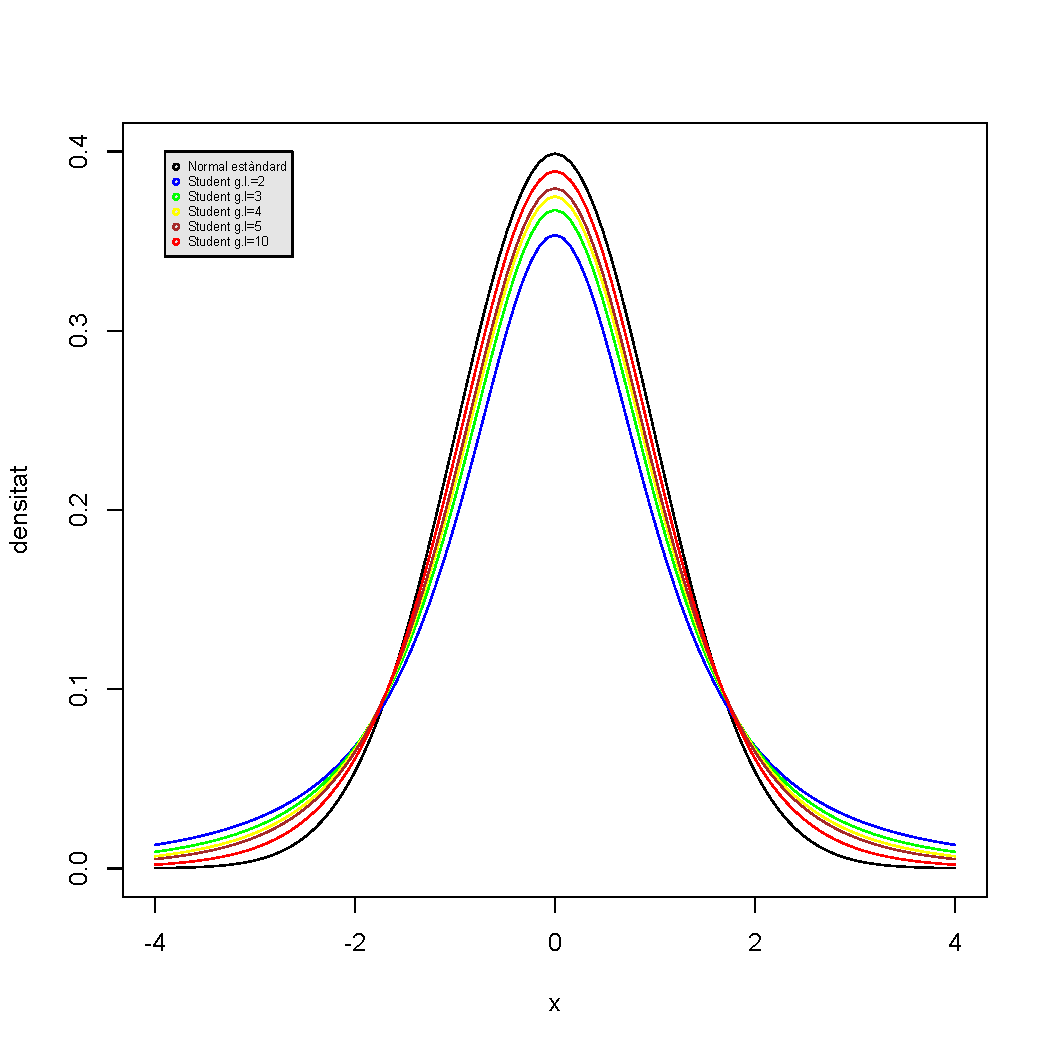
\includegraphics[width=0.95\linewidth]{tstud-div.pdf}
\end{frame}



\begin{frame}
\frametitle{Distribución $t$ de Student}

Indicaremos con
\red{$t_{\nu,q}$} el  $q$-cuantil de una  v.a.  $X_{t_{\nu}}$ que sigue una distribución $t_\nu$:
$$
P(X_{t_{\nu}}\leq t_{\nu,q})=q
$$

Por simetría,
\red{$t_{\nu,q}=-t_{\nu,1-q}$}
\vspace*{-1ex}

\begin{center}
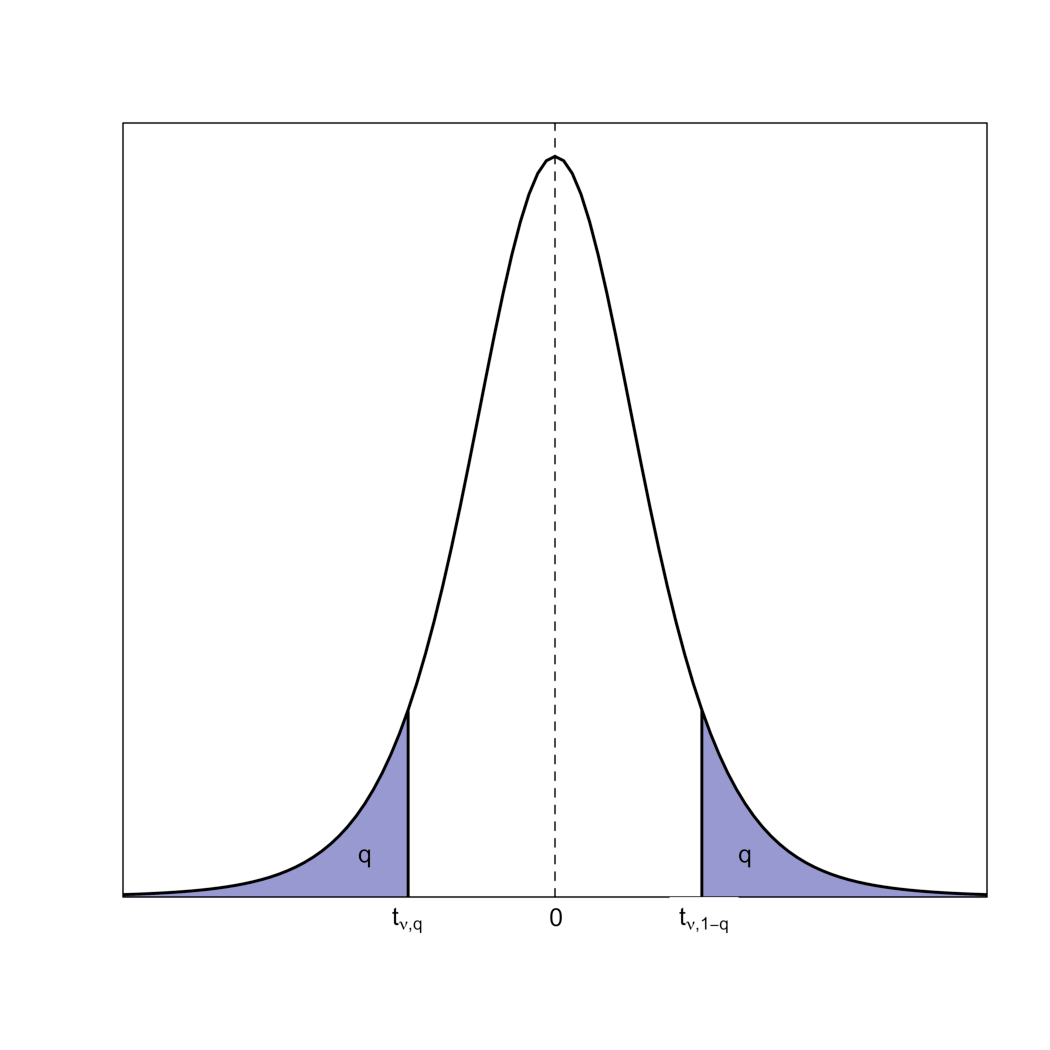
\includegraphics[width=0.6\linewidth]{quantilt}
\end{center}
\end{frame}



\begin{frame}
\frametitle{$\mu$ de población normal con $\sigma$ desconocida}

Consideremos  la situación siguiente  :
\begin{itemize}
\item  $X$ una v.a.  normal con $\mu$ y $\sigma$ desconocidas

\item $X_1,\ldots,X_n$ una m.a.s. de $X$  de  tamaño  $n$, con media   $\overline{X}$ y varianza muestral $\widetilde{S}_X^2$
\end{itemize}


\begin{teorema}
En estas  condicions, un intervalo  de confianza  del $(1-\alpha)\cdot 100\%$ I.C. para $\mu$ de una población normal con $\sigma$ conocida $\mu$
es 
$$
\left] 
\overline{X}-t_{n-1,1-\frac{\alpha}{2}} \frac{\widetilde{S}_{X}}{\sqrt{n}},
\overline{X}+t_{n-1,1-\frac{\alpha}{2}}\frac{\widetilde{S}_{X}}{\sqrt{n}} \right[
$$
\end{teorema}

\end{frame}

%
%
%\begin{frame}[fragile]
%\frametitle{$\mu$ de població normal con $\sigma$ desconocida}
%\vspace*{-5ex}
%
%\small
%\begin{verbatim}
%ICT=function(x,alpha){
%c(mean(x)-qt(1-alpha/2,length(x)-1)
%  *sd(x)/sqrt(length(x)),
%mean(x)+qt(1-alpha/2,length(x)-1)
%  *sd(x)/sqrt(length(x)))}
%set.seed(5)
%mu=1.5; sigma=0.4; alpha=0.05
%Poblacio=rnorm(10^6,mu,sigma)
%M=replicate(100,ICT(sample(Poblacio,15,replace=T),
%  alpha))
%plot(1:10,type="n",xlim=c(1.2,1.8),ylim=c(0,100),
%xlab="Valors",ylab="Replicacions")
%for(i in 1:100){color="grey";
%if((mu<M[1,i]) | (mu > M[2,i])){color = "red"}
%segments(M[1,i],i,M[2,i],i,col=color,lwd=3)}
%abline(v=mu,lwd=3)
%\end{verbatim}
%\end{frame}
%
%\begin{frame}
%\frametitle{$\mu$ de població normal con $\sigma$ desconocida}
%\vspace*{-1.2cm}
%
%\begin{center}
%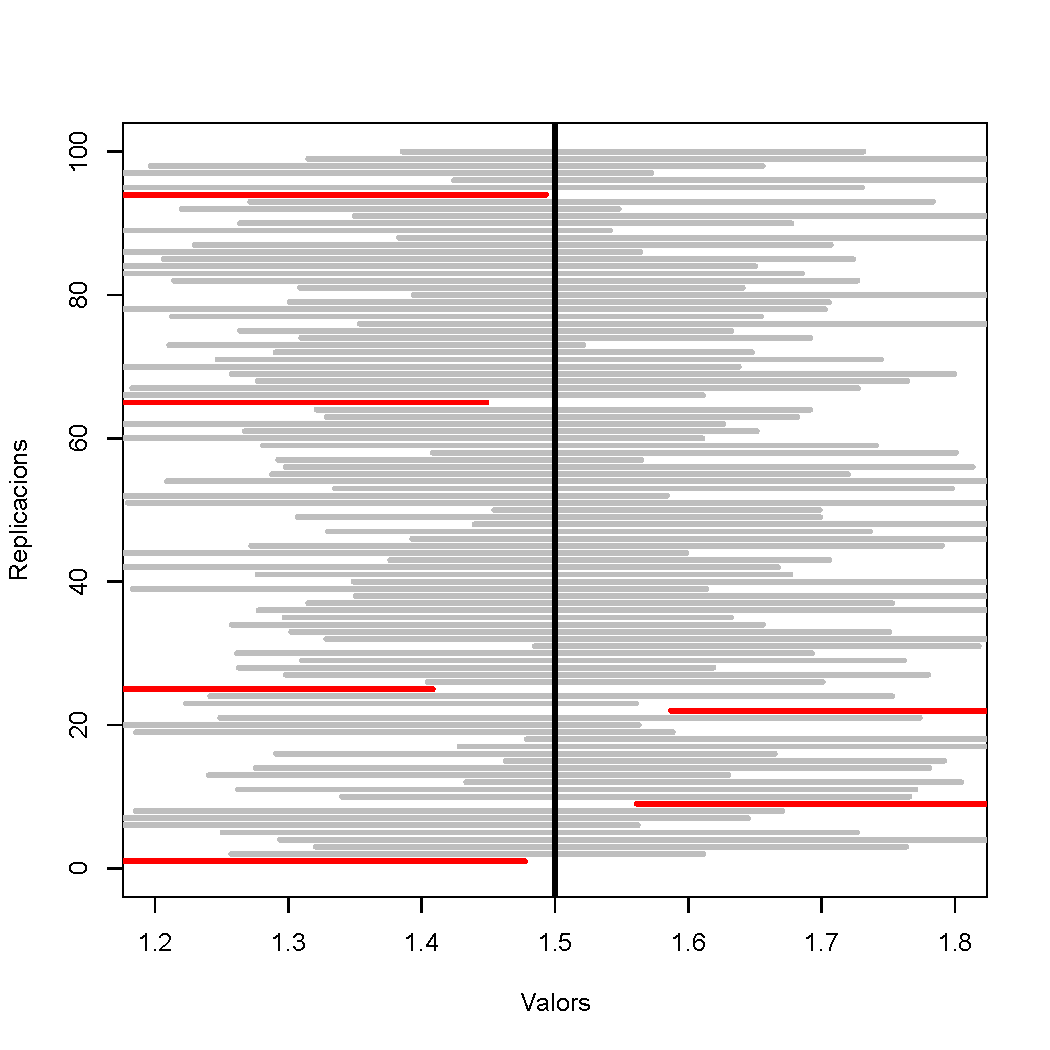
\includegraphics[width=0.9\linewidth]{intervals2}
%\end{center}
%\end{frame}
%
%
%
%




\begin{frame}
\frametitle{Ejemplo}

La empresa \textsl{3D-print} ofrece una impresora industrial de papel en color de alta capacidad. En su publicidad afirma que sus cartuchos imprimen una media de 500 mil copias con la especificación: 
\medskip

\blue{\texttt{Datos tècnicos: Muestra de  tamaño  $n=100$,
población aproximadamente normal, nivel de confianza  del 90\%}}
\medskip 

La OCU (asociación de consumidores) desea comprobar estas  afirmaciones y su laboratorio toma una muestra aleatoria de  tamaño  $n=24$, obteniendo una media   de $\overline{x}=518$ mil impresiones y una desviación típica muestral $\widetilde{s}=40$
\medskip

¿Con esta muestra, la media   poblacional anunciada per fabricante cae en el  intervalo de confianza  del 90\%?
\end{frame}

\begin{frame}[fragile]
\frametitle{Ejemplo}
Cal calcular el intervalo de confianza  I.C. para $\mu$ de población normal con $\sigma$ conocida$\mu$ con 
$$
n=24, \overline{x}=518, \widetilde{s}=40, \alpha=0.1
$$
Será
$$
\left] 
\overline{x}-t_{24,0.95} \frac{\widetilde{s}}{\sqrt{n}},
\overline{x}+t_{24,0.95} \frac{\widetilde{s}}{\sqrt{n}}\right[
$$
Consultando las tablas de la distribución  $t$ de Student, Obtenemos $t_{24,0.95}=1.71$

\begin{knitrout}\small
\definecolor{shadecolor}{rgb}{0.969, 0.969, 0.969}\color{fgcolor}\begin{kframe}
\begin{alltt}
\hlkwd{qt}\hlstd{(}\hlnum{0.95}\hlstd{,}\hlnum{24}\hlstd{)}
\end{alltt}
\begin{verbatim}
## [1] 1.710882
\end{verbatim}
\begin{alltt}
\hlkwd{round}\hlstd{(}\hlkwd{qt}\hlstd{(}\hlnum{0.95}\hlstd{,}\hlnum{24}\hlstd{),}\hlnum{2}\hlstd{)}
\end{alltt}
\begin{verbatim}
## [1] 1.71
\end{verbatim}
\end{kframe}
\end{knitrout}




Operant: $]531.962,504.038[$, y no contien a 500 (¡pero se equivoca a favor del consumidor!)
\end{frame}

\begin{frame}
\frametitle{Observaciones }

\begin{itemize}
\item el intervalo de confianza  obtenido  está centrado   en $\overline{X}$
\medskip

\item La fórmula
$$
\left] 
\overline{X}-t_{n-1,1-\frac{\alpha}{2}} \frac{\widetilde{S}_{X}}{\sqrt{n}},
\overline{X}+t_{n-1,1-\frac{\alpha}{2}}\frac{\widetilde{S}_{X}}{\sqrt{n}} \right[
$$

I.C. para $\mu$ de población normal con $\sigma$ conocida el   intervalo de confianza  del $(1-\alpha)\cdot 100\%$ se  puede utilizar  cuando $X$ es normal y $n$ cualquiera
\bigskip

\item Si $n$ es grande $t_{n-1,1-\frac{\alpha}{2}}\approx z_{1-\frac{\alpha}{2}}$ y podemos \emph{aproximarlo}  mediante
$$
\left] 
\overline{X}-z_{1-\frac{\alpha}{2}} \frac{\widetilde{S}_{X}}{\sqrt{n}},
\overline{X}+z_{1-\frac{\alpha}{2}}\frac{\widetilde{S}_{X}}{\sqrt{n}} \right[
$$
\end{itemize}


\end{frame}







\subsection{$\mu$ I.C. para $\mu$ de población normal con $\sigma$ conocida muestra grande}

\begin{frame}
\frametitle{$\mu$ I.C. para $\mu$ de población normal con $\sigma$ conocida muestras grande}

Consideremos la situación siguiente  :
\begin{itemize}
\item  $X$ una v.a.  \emph{cualquiera} con media   poblacional $\mu$ desconocida y desv. típ. $\sigma$ conocida

\item $X_1,\ldots,X_n$ una m.a.s. de $X$, con media   $\overline{X}$

\item \emph{$n$ es grande} (pongamos que $n\geq 40$)
\end{itemize}

\only<2>{En estas  condicions (T.C.L.)
$$
\frac{\overline{X}-\mu}{\frac{\sigma}{\sqrt{n}}}\approx N(0,1)
$$}

\only<3>{\begin{teorema}
En estas  condiciones, podemos tomar como intervalo  de confianza  del $(1-\alpha)\cdot 100\%$ I.C. para $\mu$ de población normal con $\sigma$ conocida $\mu$
$$
\left]\overline{X}-z_{1-\frac{\alpha}{2}}\frac{\sigma}{\sqrt{n}},
    \overline{X}+z_{1-\frac{\alpha}{2}}\frac{\sigma}{\sqrt{n}}\right[
$$
\end{teorema}}



\end{frame}


\begin{frame}
\frametitle{$\mu$ I.C. para $\mu$ de población normal con $\sigma$ conocida muestra grande}

Consideremos  la situación siguiente  :
\begin{itemize}
\item  $X$ una v.a.  \emph{cualquiera} con media   poblacional $\mu$ desconocida  \emph{y desv. típ. $\sigma$ desconocida}

\item $X_1,\ldots,X_n$ una m.a.s. de $X$, con media   $\overline{X}$ \emph{y desviación típica muestral $\widetilde{S}_X$}

\item \emph{$n$ es grande} (pogamos que $n\geq 40$)
\end{itemize}
%\pause


\begin{block}{``Teorema''}
En estas  condiciones, se recomienda tomar como  intervalo  de
confianza  del $(1-\alpha)\cdot 100\%$  para $\mu$ de población normal con $\sigma$ conocida $\mu$
$$
\left]\overline{X}-z_{1-\frac{\alpha}{2}}\frac{\widetilde{S}_X}{\sqrt{n}},
    \overline{X}+z_{1-\frac{\alpha}{2}}\frac{\widetilde{S}_X}{\sqrt{n}}\right[
$$
\end{block}



\end{frame}

%
%\begin{frame}[fragile]
%\frametitle{$\mu$ I.C. para $\mu$ de población normal con $\sigma$ conocidamostres grans}
%\vspace*{-2ex}
%
%\small
%\begin{verbatim}
%ICZ2=function(x,alpha){
%  c(mean(x)-qnorm(1-alpha/2)*sd(x)/sqrt(length(x)), 
%  mean(x)+qnorm(1-alpha/2)*sd(x)/sqrt(length(x)))
%}
%set.seed(15)
%lconda=1.5; alpha=0.05
%Poblacio=rpois(10^6,lconda)
%M=replicate(100,ICZ(sample(Poblacio,40,replace=T),
%  alpha))
%plot(1:10,lwd=3,xlim=c(1.2,1.8),ylim=c(0,100),
%xlab="Valors",ylab="Replicacions")
%for(i in 1:100){
%  color="grey";
%  if((mu<M[1,i]) | (mu > M[2,i])){color = "red"}
%  segments(M[1,i],i,M[2,i],i,col=color,lwd=3)
%}
%abline(v=mu,lwd=3)
%\end{verbatim}
%\end{frame}
%
%\begin{frame}
%\frametitle{$\mu$ I.C. para $\mu$ de población normal con $\sigma$ conocidamostres grans}
%\vspace*{-1.2cm}
%
%\begin{center}
%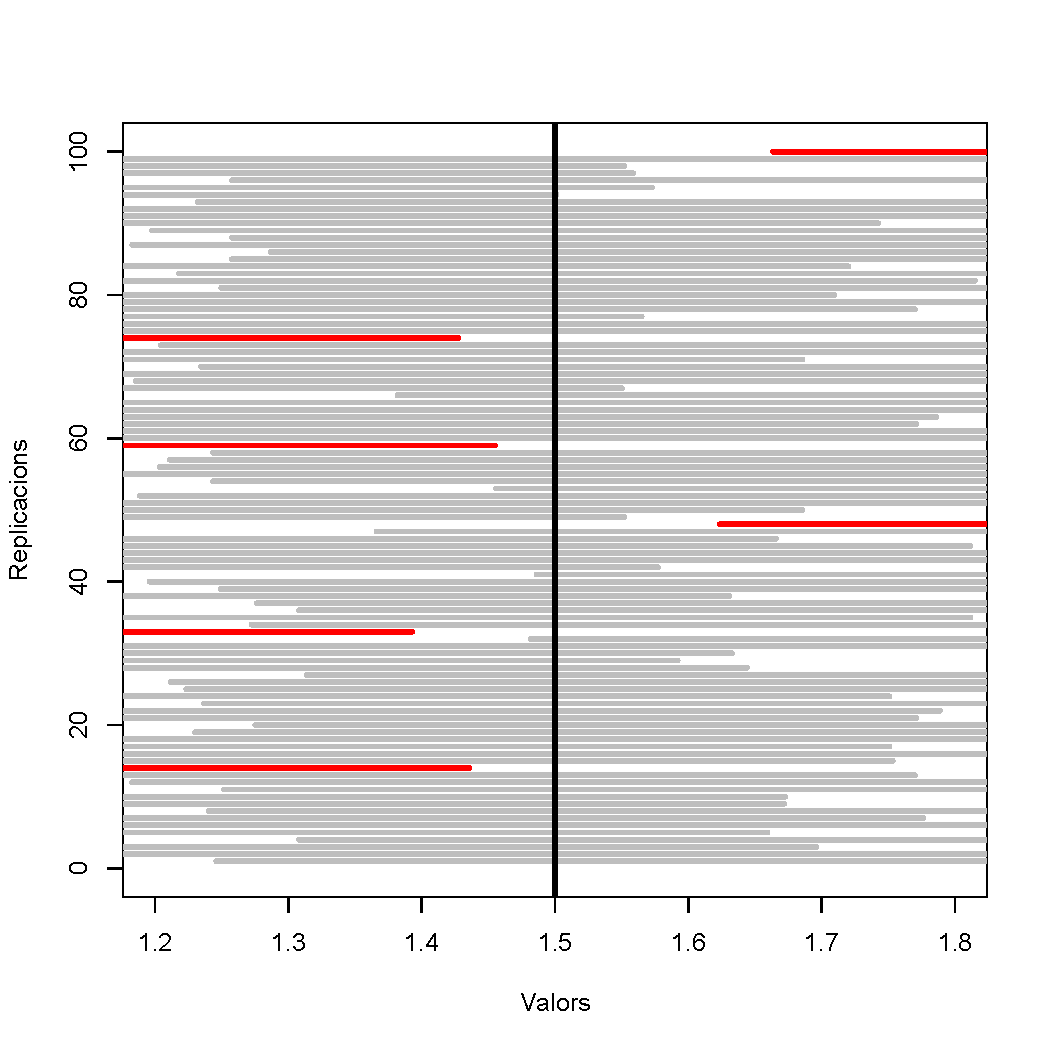
\includegraphics[width=0.9\linewidth]{intervals3}
%\end{center}
%\end{frame}
%





\begin{frame}[fragile]
\frametitle{Ejemplo}
\vspace*{-2ex}
%\MYhref[brown]{http://www.google.com}{Google}
La \MYhref[green]{https://twitter.com/guardiacivil/status/805154653977608192/photo/1}{Guardia civil informa...}
En un experimento se ha medido la tasa oficial  de  alcoholemia en sangre a 40 varones (sobrios) después de tomar 3 cañas de cerveza de 330 ml La media  y la desviació típica muestral de  porcentajes .
El siguiente código simula este experimento supuesto que la tasa

\begin{knitrout}
\definecolor{shadecolor}{rgb}{0.969, 0.969, 0.969}\color{fgcolor}\begin{kframe}
\begin{alltt}
\hlstd{tasa_alcoholemia}\hlkwb{=}\hlkwd{round}\hlstd{(}\hlkwd{rnorm}\hlstd{(}\hlnum{40}\hlstd{,}\hlkwc{mean}\hlstd{=}\hlnum{0.7}\hlstd{,}\hlkwc{sd}\hlstd{=}\hlnum{0.1}\hlstd{),}\hlnum{2}\hlstd{)}
\hlstd{tasa_alcoholemia}
\end{alltt}
\begin{verbatim}
##  [1] 0.66 0.71 0.54 0.55 0.62 0.75 0.83 0.82 0.59 0.79 0.62 0.72 0.77 0.77
## [15] 0.90 0.51 0.68 0.61 0.76 0.65 0.73 0.67 0.61 0.58 0.80 0.78 0.69 0.59
## [29] 0.92 0.66 0.69 0.64 0.62 0.67 0.75 0.70 0.72 0.71 0.79 0.60
\end{verbatim}
\end{kframe}
\end{knitrout}



$$
\overline{x}=41.2,\quad \widetilde{s}=2.1
$$
\blue{Calculad  un intervalo del que podamos afirmar que con una probabilidad del 95\% contiene el porcentaje de aumento medio de alcohol en sangre de una persona después de beber cuatro cañas de cerveza}
\medskip
%\pause

\end{frame}

%\end{document}
\begin{frame}
\frametitle{Ejemplo}


Nos piden un \emph{intervalo de confianza  del 95\%}  para $\mu$ de población normal con $\sigma$ conocida $\mu$ de la v.a. $X$ ``porcentaje de aumento de alcohol en sangre después de una persona después de  beber cuatro cañas de cerveza''

No conocemos la distribución de  $X$, pero $n=40$ es "grande"
\end{frame}

\begin{frame}
\frametitle{Ejemplo}
Podemos emplear
$$
\left]\overline{x}-z_{1-\frac{\alpha}{2}}\frac{\widetilde{s}}{\sqrt{n}},
    \overline{x}+z_{1-\frac{\alpha}{2}}\frac{\widetilde{s}}{\sqrt{n}}\right[
$$
on
$$
\begin{array}{c}
n=40,\overline{x}=41.2,\widetilde{s}=2.1,\\[1ex]
\alpha=0.05\Rightarrow z_{1-\frac{\alpha}{2}}=z_{0.975}=1.96
\end{array}
$$
\pause
$$
]40.55, 41.85[
$$

Podemos afirmar con un 95\% de confianza  que el porcentaje medio de  aumento de alcohol en sangre de una persona después de beber cuatro cañas de cerveza está entre el $40.55\%$ y el $41.85\%$


\end{frame}



\begin{frame}
\frametitle{Ejemplo}
\vspace*{-2ex}

S'ha pres una mostra de sang a 1000 adults sans y s'hi ha mesurat la quantitat  de calci (en mg per dl de sang). S'ha obtenido  una media   muestral de 9.5 mg/dl con una desviació típica muestral de 0.5 mg/dl. 
\medskip

\blue{Trobau un intervalo de confianza  del 95\% I.C. para $\mu$ de población normal con $\sigma$ conocidala quantitat media   de calci en sang en un adult sa}

\end{frame}


\begin{frame}
\frametitle{Ejemplo}
\vspace*{-2ex}

Com que $n=1000$ es grande, podem emprar
$$
\left]\overline{x}-z_{1-\frac{\alpha}{2}}\frac{\widetilde{s}}{\sqrt{n}},
    \overline{x}+z_{1-\frac{\alpha}{2}}\frac{\widetilde{s}}{\sqrt{n}}\right[
$$
on
$$
\overline{x}=9.5,\ \widetilde{s}=0.5,\
\alpha=0.05,\  z_{1-\frac{\alpha}{2}}=z_{0.975}=1.96
$$
Dóna
$$
]9.47, 9.53[
$$

Podem afirmar con un 95\% de confianza  que la quantitat media   de calci en sang en un adult sa está entre  $9.47$  y  $9.53$ mg/dl


\end{frame}



\begin{frame}
\frametitle{Amplitud}
\vspace*{-2ex}

L'Amplitud de 
$$
\left]\overline{X}-z_{1-\frac{\alpha}{2}}\frac{\widetilde{S}_X}{\sqrt{n}},
    \overline{X}+z_{1-\frac{\alpha}{2}}\frac{\widetilde{S}_X}{\sqrt{n}}\right[
$$
es
$$
A=2z_{1-\frac{\alpha}{2}}\frac{\widetilde{S}_X}{\sqrt{n}}
$$
Per determinar $n$ (gran) que doni com a màxim una Amplitud $A$ prefixada, ens cal $\widetilde{S}_X$, que depèn de la mostra.
\medskip

 Solucions:
\begin{itemize}
\item Si sabem la desv. típ. poblacional $\sigma$, l'empram en lloc de $\widetilde{S}_X$

\item Si hem pres una mostra prèvia (\emph{pilot}), n'empram la desviació típica muestral per estimar $\sigma$

\end{itemize}



\end{frame}



\begin{frame}
\frametitle{Amplitud}

\begin{block}{}
D'una població $X$ n'hem pres una  \emph{m.a.s.\ pilot} que ha tingut una desviació típica muestral $\widetilde{s}_{pilot}$.
\medskip

Estimarem que la  tamaño  mínima $n$ de una m.a.s.\ de $X$ que doni un intervalo de confianza  I.C. para $\mu$ de población normal con $\sigma$ conocida$\mu_X$ de nivell de confianza  $1-\alpha$ y Amplitud màxima $A_0$ es 
$$
n=\left\lceil \Big(2z_{1-\frac{\alpha}{2}}\frac{\widetilde{s}_{pilot}}{A_0}\Big)^2\right\rceil
$$
\end{block}



\end{frame}





\begin{frame}
\frametitle{Ejemplo}

Volem estimar l'alçada media   dels estudiants de la UIB. Cercam  un intervalo de confianza  del 99\% con una precisió màxima de 1 cm. En una mostra pilot de 25 estudiants, obtinguérem 
$$
\overline{x} = 170\mbox{ cm}, \widetilde{s}=10\mbox{ cm}
$$
Basant-nos en estas  dades, quina  tamaño  hauria de tenir la mostra per assolir el nostre objectiu?

\end{frame}


\begin{frame}
\frametitle{Ejemplo}

$$
n=
\left\lceil \Big(2z_{1-\frac{\alpha}{2}}\frac{\widetilde{s}_{pilot}}{A}\Big)^2\right\rceil=
\left\lceil \Big(z_{1-\frac{\alpha}{2}}\frac{\widetilde{s}_{pilot}}{A/2}\Big)^2\right\rceil
$$

\begin{itemize}
\item Precisió = error màxim = ${A}/{2}=1$
\medskip

\item $\widetilde{s}_{pilot}=10$
\medskip

\item $\alpha=0.01\Rightarrow z_{1-\frac{\alpha}{2}}=z_{0.995}=2.58$
\end{itemize}
Dóna
$$
n=\left\lceil \Big(2.58\cdot \frac{10}{1}\Big)^2\right\rceil=\lceil 665.64\rceil=666
$$

\end{frame}



\subsection{$p$ I.C. para $\mu$ de población normal con $\sigma$ conocidamostres petites}


\begin{frame}
\frametitle{$p$ I.C. para $\mu$ de población normal con $\sigma$ conocidamostres petites}

Consideremos la situación siguiente  :
\begin{itemize}
\item  $X$ una v.a. Bernoulli con $p$ desconocida

\item $X_1,\ldots,X_n$ una m.a.s. de $X$, con nombre d'èxits $x$ y per tant freqüència relativa d'èxits $\widehat{p}_{X}=x/n$
\end{itemize}

Recordau que $x$ es$B(n,p)$

\begin{block}{Mètode ``exacte'' de Clopper-Pearson}
Un intervalo de confianza  $]p_0,p_1[$ del $(1-\alpha)100\%$ I.C. para $\mu$ de población normal con $\sigma$ conocida$p$ s'obté trobant el $p_0$ mes grande y el $p_1$ mespetit tals que
$$
\displaystyle\sum_{k=x}^np_0^k(1-p_0)^{n-k}\leq \frac{\alpha}{2},\qquad
\displaystyle\sum_{k=0}^xp_1^k(1-p_1)^{n-k}\leq \frac{\alpha}{2}
$$
\end{block}
A mà (consultant taules) esuna feinada.

\end{frame}



\begin{frame}[fragile]
\frametitle{$p$ I.C. para $\mu$ de población normal con $\sigma$ conocidamostres petites}
\vspace*{-2ex}

El paquet \texttt{epitools} porta
\begin{center}
{\tt binom.exact(èxits, tamaño ,conf.)}
\end{center}
per calcular-ho.
\medskip

\blue{De 10 pacients tractats con un medicament, 2 s'han curat. Donau un intervalo de confianza  del 95\% I.C. para $\mu$ de población normal con $\sigma$ conocidala proporció $p$ de pacients que aquest medicament cura.}
\begin{verbatim}
> install.packages("epitools",dep=TRUE)
> library(epitools)
> round(binom.exact(2,10,0.95),3)
  x  n proportion lower upper conf.level
1 2 10        0.2 0.025 0.556       0.95
\end{verbatim}
Dóna $]0.025,0.556[$
\end{frame}

\subsection{$p$ I.C. para $\mu$ de población normal con $\sigma$ conocidamostres grans}


\begin{frame}
\frametitle{$p$ I.C. para $\mu$ de población normal con $\sigma$ conocidamostres grans I}

Consideremos ara la situación siguiente  :
\begin{itemize}
\item  $X$ una v.a. Bernoulli con $p$ desconocida

\item $X_1,\ldots,X_n$ una m.a.s. de $X$, con $n$  gran (per Ejemplo, $n\geq 40$) y freqüència relativa d'èxits $\widehat{p}_{X}$
\end{itemize}
\medskip

En estas  condicions (pel T.C.L.), 
$$
Z=\dfrac{\widehat{p}_{X}-p}
{\sqrt{\frac{p(1-p)}{n}}}\approx N(0,1)
$$
\end{frame}


\begin{frame}
\frametitle{$p$ I.C. para $\mu$ de población normal con $\sigma$ conocidamostres grans I}
Per tant
$$
P\left(-z_{1-\frac{\alpha}{2}}\leq \dfrac{\widehat{p}_{X}-p}
{\sqrt{\frac{p(1-p)}{n}}}\leq z_{1-\frac{\alpha}{2}}\right)=1-\alpha
$$
i aïllant la $p$ Obtenimos:
\end{frame}


\begin{frame}
\frametitle{$p$ I.C. para $\mu$ de población normal con $\sigma$ conocidamostres grans I}
\begin{block}{Mètode de Wilson}
En estas  condicions, un intervalo  de confianza  del $(1-\alpha)\cdot 100\%$ I.C. para $\mu$ de población normal con $\sigma$ conocida$p$
es (posant $\widehat{q}_{X}=1-\widehat{p}_{X}$)
$$
\begin{array}{l}
\displaystyle \left]\frac{\widehat{p}_{X}+\frac{z_{1-{\alpha}/{2}}^2}{2n}-z_{1-{\alpha}/{2}}\sqrt{\frac{\widehat{p}_{X}\widehat{q}_{X}}{n}+\frac{z_{1-{\alpha}/{2}}^2}{4n^2}}}{1+\frac{z_{1-{\alpha}/{2}}^2}{n}}\right.,\\[2ex]
\hspace*{2cm} \displaystyle \left.\frac{\widehat{p}_{X}+\frac{z_{1-{\alpha}/{2}}^2}{2n}+z_{1-{\alpha}/{2}}\sqrt{\frac{\widehat{p}_{X}\widehat{q}_{X}}{n}+\frac{z_{1-{\alpha}/{2}}^2}{4n^2}}}{1+\frac{z_{1-{\alpha}/{2}}^2}{n}}\right[
\end{array}
$$
\end{block}
\medskip

\texttt{binom.wilson} del paquet \texttt{epitools}
\end{frame}



\begin{frame}
\frametitle{$p$ I.C. para $\mu$ de población normal con $\sigma$ conocidamostres grans II}

Consideremos ara la situación siguiente  :
\begin{itemize}
\item  $X$ una v.a. Bernoulli con $p$ desconocida

\item $X_1,\ldots,X_n$ una m.a.s. de $X$, con $n$ mes grande y $\widehat{p}_{X}$ enfora de 0 y 1. Per Ejemplo, tal que:
$$
n\geq 100, n\widehat{p}_{X}\geq 10,  n(1-\widehat{p}_{X})\geq 10
$$
\end{itemize}
\medskip



\begin{block}{Fórmula de Laplace (1812)}
En estas  condicions, es pot prendre com a intervalo  de confianza  del $(1-\alpha)\cdot 100\%$ I.C. para $\mu$ de población normal con $\sigma$ conocida$p$
$$
\left]\widehat{p}_{X}-z_{1-\frac{\alpha}{2}}\sqrt{\frac{\widehat{p}_{X}
(1-\widehat{p}_{X})}{n}},
\widehat{p}_{X}+z_{1-\frac{\alpha}{2}}\sqrt{\frac{\widehat{p}_{X}
(1-\widehat{p}_{X})}{n}}\right[$$
\end{block}
\end{frame}



\begin{frame}
\frametitle{Ejemplo}

En una mostra aleatòria de 500 famílies con nins en edat escolar es
va trobar que 340 introduïen fruita de forma diària en la dieta dels seus fills
\medskip

Cercau un intervalo de confianza  del 95\% I.C. para $\mu$ de población normal con $\sigma$ conocidala proporció real de
famílies d'aquesta ciutat con nins en edat escolar que incorporen fruita fresca de
forma diària en la dieta dels seus fills


\end{frame}
\begin{frame}
\frametitle{Ejemplo}

$X=$ ``Aportar diàriament fruita a la dieta dels fills''\\
 es$Be(p)$, y cercam intervalo de confianza  del 95\% I.C. para $\mu$ de población normal con $\sigma$ conocida$p$
\bigskip

Com que $n=500\geq 100$, $n\widehat{p}_X=340\geq 10$ y $n(1-\widehat{p}_X)=160\geq 10$, podem emprar
$$
\left]\widehat{p}_{X}-z_{1-\frac{\alpha}{2}}\sqrt{\frac{\widehat{p}_{X}
(1-\widehat{p}_{X})}{n}},
\widehat{p}_{X}+z_{1-\frac{\alpha}{2}}\sqrt{\frac{\widehat{p}_{X}
(1-\widehat{p}_{X})}{n}}\right[
$$
con
$$
n=500, \widehat{p}_{X}=\dfrac{340}{500}=0.68
$$
Dóna (recordau $\alpha=0.05\Rightarrow z_{1-\frac{\alpha}{2}}=z_{0.975}=1.96$)
$$
\red{]0.639,0.721[}
$$

\end{frame}

\begin{frame}[fragile]
\frametitle{Ejemplo}

Con els altres mètodes:
\begin{verbatim}
> round(binom.exact(340,500,0.95),3)
    x   n proportion lower upper conf.level
1 340 500       0.68 0.637 0.721       0.95
> round(binom.wilson(340,500,0.95),3)
    x   n proportion lower upper conf.level
1 340 500       0.68 0.638 0.719       0.95
\end{verbatim}
Donen:
\medskip

\begin{itemize}
\item Clopper-Pearson: $]0.637,0.721[$
\medskip

\item Wilson: $]0.638, 0.719[$
\medskip

\item Laplace: $]0.639,0.721[$
\end{itemize}

\end{frame}

\begin{frame}
\frametitle{Ejemplo}

\blue{En un assaig d'un nou tractament de quimioteràpia, en una mostra de $n$ (gran) malalts tractats, cap desenvolupà càncer testicular com a efecte secundari. Trobau un intervalo de confianza  al 95\% I.C. para $\mu$ de población normal con $\sigma$ conocidala proporció de malalts tractats con aquesta quimio que desenvolupen càncer testicular.}
\pause\bigskip

No podem emprar la fórmula de Laplace, perquè $\widehat{p}_X=0$. Cal emprar el mètode de Wilson:


\end{frame}

\begin{frame}
\frametitle{Ejemplo}
\vspace*{-5ex}

{\small
$$
\begin{array}{l}
\displaystyle \left]\frac{\widehat{p}_{X}+\frac{z_{1-{\alpha}/{2}}^2}{2n}-z_{1-{\alpha}/{2}}\sqrt{\frac{\widehat{p}_{X}\widehat{q}_{X}}{n}+\frac{z_{1-{\alpha}/{2}}^2}{4n^2}}}{1+\frac{z_{1-{\alpha}/{2}}^2}{n}}\right.,\\[2ex]
\hspace*{2cm} \displaystyle \left.\frac{\widehat{p}_{X}+\frac{z_{1-{\alpha}/{2}}^2}{2n}+z_{1-{\alpha}/{2}}\sqrt{\frac{\widehat{p}_{X}\widehat{q}_{X}}{n}+\frac{z_{1-{\alpha}/{2}}^2}{4n^2}}}{1+\frac{z_{1-{\alpha}/{2}}^2}{n}}\right[
\end{array}
$$
\pause
$$
\left]\frac{\frac{1.96^2}{2n}- 1.96\sqrt{\frac{1.96^2}{4n^2}}}{1+\frac{1.96^2}{n}},
\frac{\frac{1.96^2}{2n}+ 1.96\sqrt{\frac{1.96^2}{4n^2}}}{1+\frac{1.96^2}{n}}\right[
=\Big]0,\frac{1.96^2}{n+1.96^2}\Big[
$$
}
\red{Els metges empren $\Big]0,\dfrac{3}{n}\Big[$ (la regla del 3)}


\end{frame}


\begin{frame}
\frametitle{Observaciones }
\begin{itemize}
\item El mètode de Wilson dóna un I.C. centrado   en
$$
\frac{\widehat{p}_{X}+\frac{z_{1-{\alpha}/{2}}^2}{2n}}{1+\frac{z_{1-{\alpha}/{2}}^2}{n}}
=\frac{2n\widehat{p}_{X}+ z_{1-\frac{\alpha}{2}}^2}{2n+2 z_{1-\frac{\alpha}{2}}^2}
$$

\item No es coneix una fórmula per al centre de l'I.C. de Clopper-Pearson.

\item La fórmula de Laplace dóna un I.C.  centrado   en $\widehat{p}_{X}$
\medskip

\item Quan $n$ creix es redueix l'Amplitud de el intervalo de confianza 

\end{itemize}

\end{frame}


\begin{frame}
\frametitle{Amplitud}

L'Amplitud de el intervalo de confianza  de Laplace es 
$$
A=2 z_{1-\frac{\alpha}{2}} \sqrt{\frac{\widehat{p}_{X} (1-\widehat{p}_{X})}{n}}
$$
No podem determinar la  tamaño  de la mostra a fi que el intervalo de confianza  tingui una certa Amplitud màxima sense
conèixer $\widehat{p}_{X}$, que no coneixem sense una mostra

\end{frame}

\begin{frame}
\frametitle{Amplitud}
\vspace*{-4ex}

$$
A=2 z_{1-\frac{\alpha}{2}} \sqrt{\frac{\widehat{p}_{X} (1-\widehat{p}_{X})}{n}}
$$
El màxim de $\sqrt{\widehat{p}_{X} (1-\widehat{p}_{X})}$ s'assoleix a $\widehat{p}_{X}=0.5$ 
\only<1>{
\begin{center}
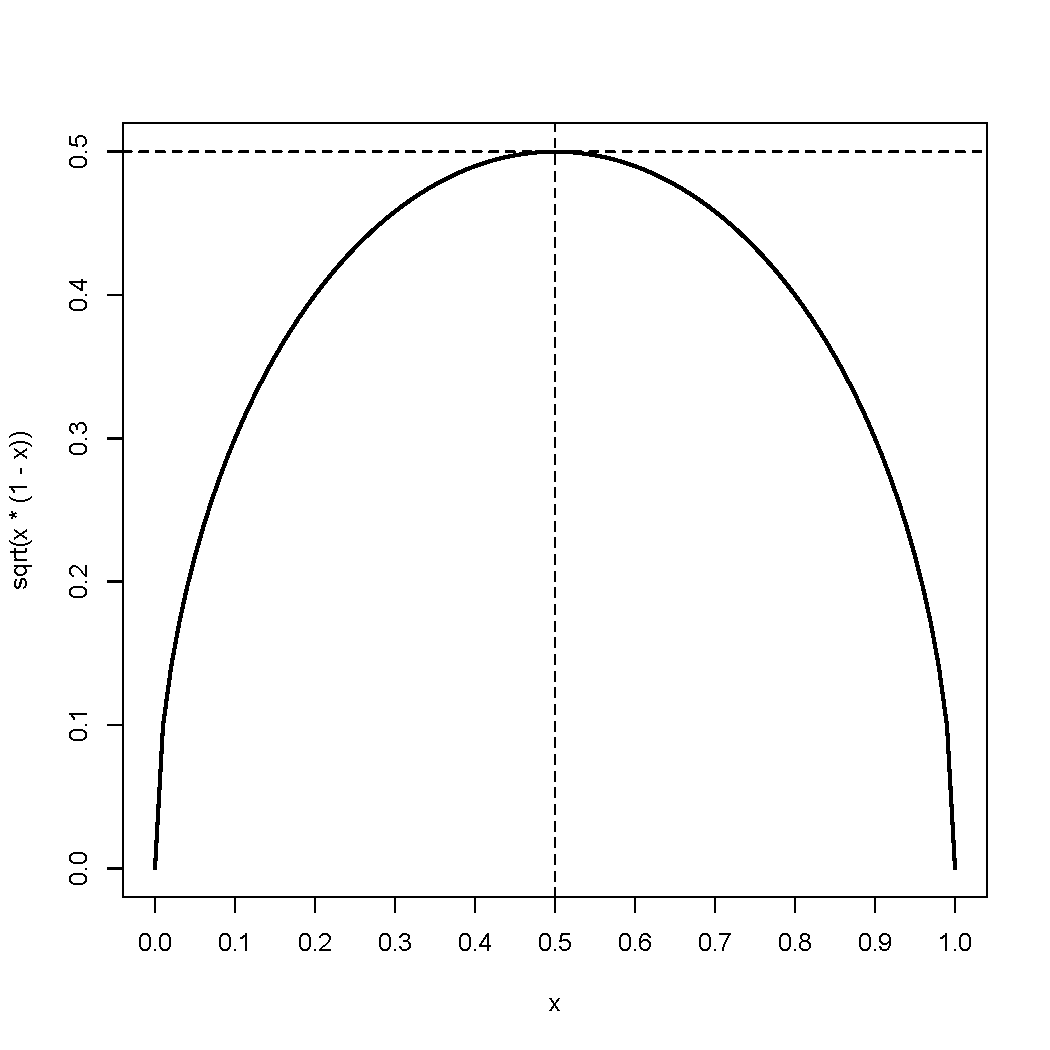
\includegraphics[width=0.6\linewidth]{p(1-p).pdf}
\end{center}}

\only<2>{\vspace*{5ex}

Per tant, calcularem $n$ per obtenir una  Amplitud com a màxim $A_0$ suposant el pitjor dels casos ($\widehat{p}_{X}=0.5$):
$$
A_0\geq 2z_{1-\frac{\alpha}{2}}\sqrt{\frac{0.5^2}{n}}=\frac{z_{1-\frac{\alpha}{2}}}{\sqrt{n}}
\Rightarrow
\red{n=\left\lceil\frac{z_{1-\frac{\alpha}{2}}^2}{A_0^2}\right\rceil}
$$}

\end{frame}


\begin{frame}
\frametitle{Ejemplos}

\begin{center}
\hspace*{-0.5cm}

\includegraphics[width=1.1\linewidth]{plagiUIB1.jpg}\bigskip

\hspace*{-0.5cm}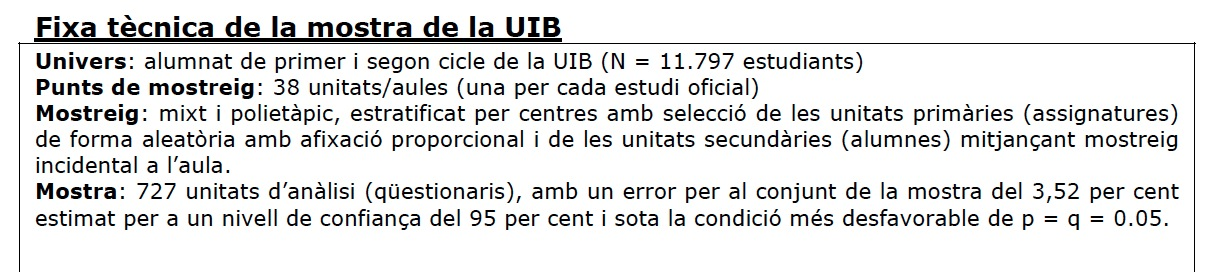
\includegraphics[width=1.1\linewidth]{plagiUIB2.jpg}
\end{center}
$$
\mbox{Error}=\pause \frac{1.96\cdot 0.5}{\sqrt{727}}\approx 0.0363
$$
\end{frame}



\begin{frame}
\frametitle{Ejemplo}
Volem estudiar quina fracció de las morts per càncer corresponen a morts per càncer d'estómac. Per determinar aquesta fracció a un nivell de confianza  del 95\% y garantir un error màxim de 0.05, de quina  tamaño  ha de ser la mostra \emph{en el pitjor dels casos}?
$$
n=\left\lceil\frac{z_{1-\frac{\alpha}{2}}^2}{A^2}\right\rceil
$$
on
$$
\frac{A}{2}=0.05,\quad z_{1-\frac{\alpha}{2}}=z_{0.975}=1.96
$$
Dóna $n= \lceil 384.16\rceil=385$.

\end{frame}




\subsection{$\sigma$ de població normal}
\begin{frame}
\frametitle{varianza de una població normal}


Consideremos ara la situación siguiente  :
\begin{itemize}
\item  $X$ una v.a. normal con $\mu$ y $\sigma$ desconocidas

\item $X_1,\ldots,X_n$ una m.a.s. de $X$ y varianza muestral $\widetilde{S}_X^2$
\end{itemize}


\begin{teorema}
En estas  condicions
$$
\frac{(n-1) \tilde{S}_{X}^2}{\sigma^2}
$$
té distribución $\chi^2_{n-1}$
\end{teorema}
\end{frame}

\begin{frame}
\frametitle{varianza de una població normal}


Consideremos ara la situación siguiente  :
\begin{itemize}
\item  $X$ una v.a. normal con $\mu$ y $\sigma$ desconocidas

\item $X_1,\ldots,X_n$ una m.a.s. de $X$ y varianza muestral $\widetilde{S}_X^2$
\end{itemize}


\begin{teorema}
En estas  condicions,  un intervalo  de confianza  del $(1-\alpha)\cdot 100\%$ I.C. para $\mu$ de población normal con $\sigma$ conocida\red{$\sigma^2$}
es 
$$
\left] \frac{(n-1)\widetilde{S}_{X}^2}{\chi_{n-1,1-\frac{\alpha}{2}}^2},
\frac{(n-1)\widetilde{S}_{X}^2}{\chi_{n-1,\frac{\alpha}{2}}^2}
\right[,
$$
on $\chi_{\nu,q}^2$ esel $q$-quantil de la distribución $\chi_{\nu}^2$
\end{teorema}
\end{frame}


\begin{frame}
\frametitle{varianza de una població normal}

En efecte
$$
\begin{array}{l}
1-\alpha=P\left(\chi_{n-1,\frac{\alpha}{2}}^2\leq \chi_{n-1}^2\leq
\chi_{n-1,1-\frac{\alpha}{2}}^2\right)\\[2ex]
\quad\displaystyle =P\left(\chi_{n-1,\frac{\alpha}{2}}^2\leq \frac{(n-1) \widetilde{S}_{X}^2}{\sigma^2}\leq
\chi_{n-1,1-\frac{\alpha}{2}}^2
\right)\\[2ex]
\quad\displaystyle = P\left(\frac{(n-1)
\widetilde{S}_{X}^2}{\chi_{n-1,1-\frac{\alpha}{2}}^2}\leq\sigma^2\leq\frac{
(n-1)\widetilde{S}_{X}^2}{\chi_{n-1,\frac{\alpha}{2}}^2}
\right)
\end{array}
$$
I ara $\chi_{n-1}^2$ no essimètrica, així que s'han de calcular $\chi_{n-1,\frac{\alpha}{2}}^2$ y $\chi_{n-1,1-\frac{\alpha}{2}}^2$
\medskip

\blue{Observació:} el intervalo de confianza  per $\sigma^2$ no està
centrado   en $\widetilde{S}_{X}^2$

\end{frame}


\begin{frame}
\frametitle{Ejemplo}

Un índex de qualitat d'un reactiu químic esel temps que triga a
actuar. L'estàndard esque aquest ha de ser $\leq 30$ segons.
Se suposa que la distribución del temps d'actuació del reactiu es 
aproximadament normal. 
\medskip


Es realitzen 30 proves en las quals es mesura el temps
d'actuació del reactiu:
\medskip

12, 13, 13, 14, 14, 14, 15, 15, 16, 17, 17, 18, 18, 19, 19, 25, 25, 26, 27, 30,
33, 34, 35, 40, 40, 51, 51, 58, 59, 83
\medskip

Es demana calcular un intervalo de confianza  I.C. para $\mu$ de población normal con $\sigma$ conocidala desviació típica al nivell
$95\%$
\end{frame}

\begin{frame}[fragile]
\frametitle{Ejemplo}
\red{$\displaystyle \left] \frac{(n-1)\widetilde{S}_{X}^2}{\chi_{n-1,1-\frac{\alpha}{2}}^2},
\frac{(n-1)\widetilde{S}_{X}^2}{\chi_{n-1,\frac{\alpha}{2}}^2}
\right[$}

\begin{verbatim}
> Temps=c(12,13,13,14,14,14,15,15,16,17,17,18,
 18,19,19,25,25,26,27,30,33,34,35,40,40,51,51,
 58,59,83)
> length(Temps) #n
[1]  30.0000
> var(Temps) # varianza mostral
[1]  301.5506
\end{verbatim}
i  $\alpha=0.05$:
$$
\chi_{29,0.975}^2=45.72,\
\chi_{29,0.025}^2=16.05
$$
\end{frame}

\begin{frame} 
\frametitle{Ejemplo}

el intervalo serà
$$
\left] \frac{(n-1)\widetilde{S}_{X}^2}{\chi_{n-1,1-\frac{\alpha}{2}}^2},
\frac{(n-1)\widetilde{S}_{X}^2}{\chi_{n-1,\frac{\alpha}{2}}^2}
\right[
$$
Obtenimos
$$
\left] \frac{29\cdot 301.5506}{45.72},
\frac{29\cdot 301.5506}{16.05}
\right[=
\red{]191.27, 544.86[}
$$
\pause

Aquest era I.C. para $\mu$ de población normal con $\sigma$ conocidala variància! I.C. para $\mu$ de población normal con $\sigma$ conocidala desviació típica
$$
]\sqrt{191.27}, \sqrt{544.86}[=\red{]13.83,23.34[}
$$

\end{frame}

\subsection{$N$ relativament petit}
\begin{frame}
\frametitle{``Poblacions finites''}
Fins ara hem emprat mostres aleatòries simples
\medskip

A la pràctica,  es prenen mostres aleatòries sense reposició
\medskip

Si la  tamaño  $N$ de la població esmolt mes grande que la  tamaño  $n$ de la mostra (posem $N\geq 40n$), las fórmules donades fins ara funcionen (aproximadament) bé
\medskip

Però\ldots
\vspace*{-4ex}

\begin{center}
\hspace*{-0.5cm}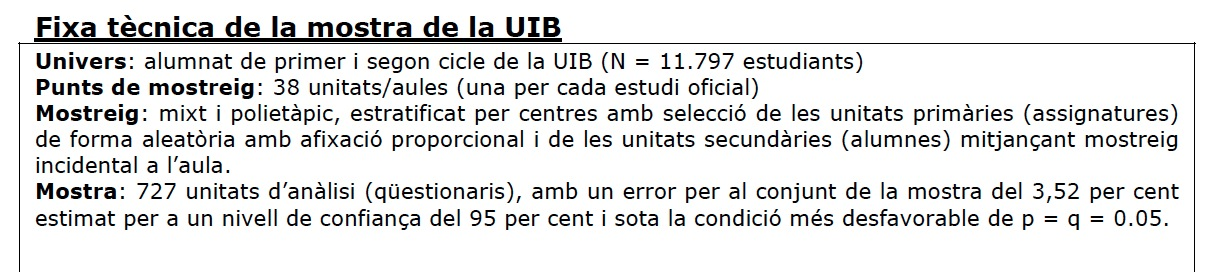
\includegraphics[width=1.1\linewidth]{plagiUIB2.jpg}
\end{center}


\end{frame}

\begin{frame}
\frametitle{``Poblacions finites''}

Es dóna l'efecte de \emph{població finita} quan $N$ esrelativament petit
\medskip

En aquest cas, a las fórmules que hem donat per als intervals de confianza  I.C. para $\mu$ de población normal con $\sigma$ conocida$\mu$ o $p$ cal multiplicar l'error estàndard o l'error muestral pel factor corrector
$$
\sqrt{\frac{N-n}{N-1}}
$$

\end{frame}

\begin{frame}
\frametitle{``Poblacions finites''}

Consideremos  la situación siguiente  :
\begin{itemize}
\item  $X$ una població de  tamaño  $N$ que sigue una distribución con media   poblacional $\mu$ desconocida

\item $X_1,\ldots,X_n$ una m.a.\ sense reposició de $X$, con media   $\overline{X}$

\item  $n$ es grande 
\end{itemize}

\begin{block}{``Teorema''}
En estas  condicions, es recomana prendre com a intervalo  de confianza  del $(1-\alpha)\cdot 100\%$ I.C. para $\mu$ de población normal con $\sigma$ conocida$\mu$
$$
\left]\overline{X}-z_{1-\frac{\alpha}{2}}\frac{\sigma}{\sqrt{n}}\sqrt{\frac{N-n}{N-1}},\
    \overline{X}+z_{1-\frac{\alpha}{2}}\frac{\sigma}{\sqrt{n}}\sqrt{\frac{N-n}{N-1}}\right[
$$
\end{block}



\end{frame}




\begin{frame}
\frametitle{``Poblacions finites''}
\vspace*{-2ex}

Consideremos  la situación siguiente  :
\begin{itemize}
\item  $X$ una població de  tamaño  $N$ que sigue una distribución Bernoulli con $p$ desconocida

\item $X_1,\ldots,X_n$ una m.a.\ sense reposició de $X$, con $n$ molt gran  y con freqüència relativa d'èxits $\widehat{p}_{X}$ no extrema
\end{itemize}
\medskip

\begin{block}{``Teorema''}
En estas  condicions, es recomana prendre com a intervalo  de confianza  del $(1-\alpha)\cdot 100\%$ I.C. para $\mu$ de población normal con $\sigma$ conocida$p$
$$
\begin{array}{l}
\displaystyle \left]\widehat{p}_{X}-z_{1-\frac{\alpha}{2}}\sqrt{\frac{\widehat{p}_{X}
(1-\widehat{p}_{X})}{n}}\sqrt{\frac{N-n}{N-1}}\right.,\\[1ex]
\hspace*{3cm}\displaystyle
\left.\widehat{p}_{X}+z_{1-\frac{\alpha}{2}}\sqrt{\frac{\widehat{p}_{X}
(1-\widehat{p}_{X})}{n}}\sqrt{\frac{N-n}{N-1}}\right[
\end{array}$$
\end{block}
\end{frame}


\begin{frame}
\frametitle{``Poblacions finites''}

\begin{block}{``Teorema''}
En las condicions anteriors, per obtenir un intervalo de confianza  del $(1-\alpha)\cdot 100\%$ I.C. para $\mu$ de población normal con $\sigma$ conocida$p$ en el pitjor dels casos caldrà prendre una mostra de  tamaño 
$$
n=\left\lceil\frac{Nz_{1-\frac{\alpha}{2}}^2}{A^2(N-1)+z_{1-\frac{\alpha}{2}}^2}\right\rceil
$$
\end{block}
\end{frame}

\begin{frame}
\frametitle{Ejemplo}
\vspace*{-5ex}

\begin{center}
\hspace*{-0.5cm}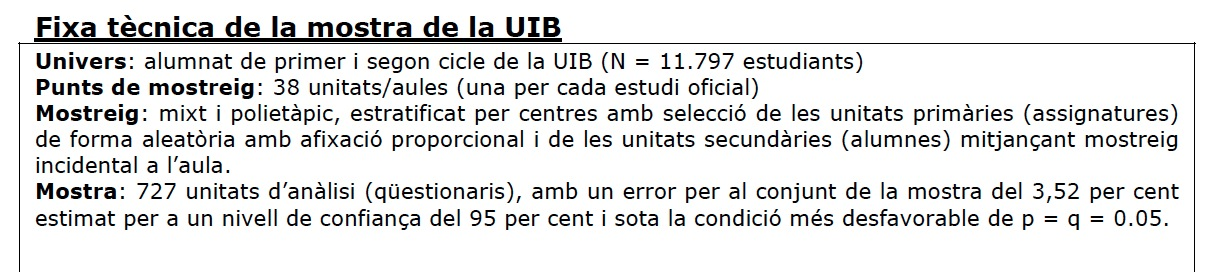
\includegraphics[width=1.1\linewidth]{plagiUIB2.jpg}
\end{center}

\blue{De la població total d'estudiants de grau de la UIB quants n'hem d'escollir de manera aleatòria sense reposició per estimar la proporció dels que han comès plagi, con un error del 3.52\% y un nivell de confianza  del 95\%?}
\pause

$$
n=\left\lceil\frac{11797\cdot 1.96^2}{0.0704^2\cdot 11796+1.96^2}\right\rceil=\lceil 727.3854\rceil=728
$$
\end{frame}

\end{document}

